% Options for packages loaded elsewhere
\PassOptionsToPackage{unicode}{hyperref}
\PassOptionsToPackage{hyphens}{url}
%
\documentclass[
  man,floatsintext]{apa7}
\usepackage{amsmath,amssymb}
\usepackage{iftex}
\ifPDFTeX
  \usepackage[T1]{fontenc}
  \usepackage[utf8]{inputenc}
  \usepackage{textcomp} % provide euro and other symbols
\else % if luatex or xetex
  \usepackage{unicode-math} % this also loads fontspec
  \defaultfontfeatures{Scale=MatchLowercase}
  \defaultfontfeatures[\rmfamily]{Ligatures=TeX,Scale=1}
\fi
\usepackage{lmodern}
\ifPDFTeX\else
  % xetex/luatex font selection
\fi
% Use upquote if available, for straight quotes in verbatim environments
\IfFileExists{upquote.sty}{\usepackage{upquote}}{}
\IfFileExists{microtype.sty}{% use microtype if available
  \usepackage[]{microtype}
  \UseMicrotypeSet[protrusion]{basicmath} % disable protrusion for tt fonts
}{}
\makeatletter
\@ifundefined{KOMAClassName}{% if non-KOMA class
  \IfFileExists{parskip.sty}{%
    \usepackage{parskip}
  }{% else
    \setlength{\parindent}{0pt}
    \setlength{\parskip}{6pt plus 2pt minus 1pt}}
}{% if KOMA class
  \KOMAoptions{parskip=half}}
\makeatother
\usepackage{xcolor}
\usepackage{graphicx}
\makeatletter
\def\maxwidth{\ifdim\Gin@nat@width>\linewidth\linewidth\else\Gin@nat@width\fi}
\def\maxheight{\ifdim\Gin@nat@height>\textheight\textheight\else\Gin@nat@height\fi}
\makeatother
% Scale images if necessary, so that they will not overflow the page
% margins by default, and it is still possible to overwrite the defaults
% using explicit options in \includegraphics[width, height, ...]{}
\setkeys{Gin}{width=\maxwidth,height=\maxheight,keepaspectratio}
% Set default figure placement to htbp
\makeatletter
\def\fps@figure{htbp}
\makeatother
\setlength{\emergencystretch}{3em} % prevent overfull lines
\providecommand{\tightlist}{%
  \setlength{\itemsep}{0pt}\setlength{\parskip}{0pt}}
\setcounter{secnumdepth}{-\maxdimen} % remove section numbering
% Make \paragraph and \subparagraph free-standing
\ifx\paragraph\undefined\else
  \let\oldparagraph\paragraph
  \renewcommand{\paragraph}[1]{\oldparagraph{#1}\mbox{}}
\fi
\ifx\subparagraph\undefined\else
  \let\oldsubparagraph\subparagraph
  \renewcommand{\subparagraph}[1]{\oldsubparagraph{#1}\mbox{}}
\fi
\newlength{\cslhangindent}
\setlength{\cslhangindent}{1.5em}
\newlength{\csllabelwidth}
\setlength{\csllabelwidth}{3em}
\newlength{\cslentryspacingunit} % times entry-spacing
\setlength{\cslentryspacingunit}{\parskip}
\newenvironment{CSLReferences}[2] % #1 hanging-ident, #2 entry spacing
 {% don't indent paragraphs
  \setlength{\parindent}{0pt}
  % turn on hanging indent if param 1 is 1
  \ifodd #1
  \let\oldpar\par
  \def\par{\hangindent=\cslhangindent\oldpar}
  \fi
  % set entry spacing
  \setlength{\parskip}{#2\cslentryspacingunit}
 }%
 {}
\usepackage{calc}
\newcommand{\CSLBlock}[1]{#1\hfill\break}
\newcommand{\CSLLeftMargin}[1]{\parbox[t]{\csllabelwidth}{#1}}
\newcommand{\CSLRightInline}[1]{\parbox[t]{\linewidth - \csllabelwidth}{#1}\break}
\newcommand{\CSLIndent}[1]{\hspace{\cslhangindent}#1}
\ifLuaTeX
\usepackage[bidi=basic]{babel}
\else
\usepackage[bidi=default]{babel}
\fi
\babelprovide[main,import]{english}
% get rid of language-specific shorthands (see #6817):
\let\LanguageShortHands\languageshorthands
\def\languageshorthands#1{}
% Manuscript styling
\usepackage{upgreek}
\captionsetup{font=singlespacing,justification=justified}

% Table formatting
\usepackage{longtable}
\usepackage{lscape}
% \usepackage[counterclockwise]{rotating}   % Landscape page setup for large tables
\usepackage{multirow}		% Table styling
\usepackage{tabularx}		% Control Column width
\usepackage[flushleft]{threeparttable}	% Allows for three part tables with a specified notes section
\usepackage{threeparttablex}            % Lets threeparttable work with longtable

% Create new environments so endfloat can handle them
% \newenvironment{ltable}
%   {\begin{landscape}\centering\begin{threeparttable}}
%   {\end{threeparttable}\end{landscape}}
\newenvironment{lltable}{\begin{landscape}\centering\begin{ThreePartTable}}{\end{ThreePartTable}\end{landscape}}

% Enables adjusting longtable caption width to table width
% Solution found at http://golatex.de/longtable-mit-caption-so-breit-wie-die-tabelle-t15767.html
\makeatletter
\newcommand\LastLTentrywidth{1em}
\newlength\longtablewidth
\setlength{\longtablewidth}{1in}
\newcommand{\getlongtablewidth}{\begingroup \ifcsname LT@\roman{LT@tables}\endcsname \global\longtablewidth=0pt \renewcommand{\LT@entry}[2]{\global\advance\longtablewidth by ##2\relax\gdef\LastLTentrywidth{##2}}\@nameuse{LT@\roman{LT@tables}} \fi \endgroup}

% \setlength{\parindent}{0.5in}
% \setlength{\parskip}{0pt plus 0pt minus 0pt}

% Overwrite redefinition of paragraph and subparagraph by the default LaTeX template
% See https://github.com/crsh/papaja/issues/292
\makeatletter
\renewcommand{\paragraph}{\@startsection{paragraph}{4}{\parindent}%
  {0\baselineskip \@plus 0.2ex \@minus 0.2ex}%
  {-1em}%
  {\normalfont\normalsize\bfseries\itshape\typesectitle}}

\renewcommand{\subparagraph}[1]{\@startsection{subparagraph}{5}{1em}%
  {0\baselineskip \@plus 0.2ex \@minus 0.2ex}%
  {-\z@\relax}%
  {\normalfont\normalsize\itshape\hspace{\parindent}{#1}\textit{\addperi}}{\relax}}
\makeatother

\makeatletter
\usepackage{etoolbox}
\patchcmd{\maketitle}
  {\section{\normalfont\normalsize\abstractname}}
  {\section*{\normalfont\normalsize\abstractname}}
  {}{\typeout{Failed to patch abstract.}}
\patchcmd{\maketitle}
  {\section{\protect\normalfont{\@title}}}
  {\section*{\protect\normalfont{\@title}}}
  {}{\typeout{Failed to patch title.}}
\makeatother

\usepackage{xpatch}
\makeatletter
\xapptocmd\appendix
  {\xapptocmd\section
    {\addcontentsline{toc}{section}{\appendixname\ifoneappendix\else~\theappendix\fi\\: #1}}
    {}{\InnerPatchFailed}%
  }
{}{\PatchFailed}
\keywords{big team, science, authorship, credit}
\usepackage{lineno}

\linenumbers
\usepackage{csquotes}
\makeatletter
\renewcommand{\paragraph}{\@startsection{paragraph}{4}{\parindent}%
  {0\baselineskip \@plus 0.2ex \@minus 0.2ex}%
  {-1em}%
  {\normalfont\normalsize\bfseries\typesectitle}}

\renewcommand{\subparagraph}[1]{\@startsection{subparagraph}{5}{1em}%
  {0\baselineskip \@plus 0.2ex \@minus 0.2ex}%
  {-\z@\relax}%
  {\normalfont\normalsize\bfseries\itshape\hspace{\parindent}{#1}\textit{\addperi}}{\relax}}
\makeatother

\ifLuaTeX
  \usepackage{selnolig}  % disable illegal ligatures
\fi
\IfFileExists{bookmark.sty}{\usepackage{bookmark}}{\usepackage{hyperref}}
\IfFileExists{xurl.sty}{\usepackage{xurl}}{} % add URL line breaks if available
\urlstyle{same}
\hypersetup{
  pdftitle={Who does big team science?},
  pdfauthor={Erin M. Buchanan1 \& Savannah C. Lewis2},
  pdflang={en-EN},
  pdfkeywords={big team, science, authorship, credit},
  hidelinks,
  pdfcreator={LaTeX via pandoc}}

\title{Who does big team science?}
\author{Erin M. Buchanan\textsuperscript{1} \& Savannah C. Lewis\textsuperscript{2}}
\date{}


\shorttitle{Big Team Science}

\authornote{

Erin M. Buchanan is a Professor of Cognitive Analytics at Harrisburg University of Science and Technology. Savannah C. Lewis is a graduate student at the University of Alabama.

Thank you to Dwayne Lieck for providing an extensive list of large scale projects for this manuscript.

Preprint: \url{https://osf.io/hqta4/}

The authors made the following contributions. Erin M. Buchanan: Conceptualization, Data curation, Formal Analysis, Methodology, Project administration, Visualization, Writing -- original draft, Writing -- review \& editing; Savannah C. Lewis: Conceptualization, Data curation, Methodology, Project administration, Writing -- original draft, Writing -- review \& editing.

Correspondence concerning this article should be addressed to Erin M. Buchanan, 326 Market St., Harrisburg, PA 17101. E-mail: \href{mailto:ebuchanan@harrisburgu.edu}{\nolinkurl{ebuchanan@harrisburgu.edu}}

}

\affiliation{\vspace{0.5cm}\textsuperscript{1} Harrisburg University of Science and Technology\\\textsuperscript{2} University of Alabama}

\abstract{%
This paper examined the nature of publications in Big Team Science (BTS): large-scale collaborations between multiple researchers at multiple institutions. These projects can improve research by initiating collaborations that span across the globe, age groups, education levels, and subfields of research. As the number of BTS publications increase, it is useful to explore who is currently involved in BTS projects to determine diversity in both research subject and researcher representation. We examined the diversity of BTS publications and authors across more than half a million articles to investigate where and what is currently published, and author characteristics including differences in career length, publication metrics, affiliation, and affiliation geopolitical regions. Interestingly, BTS publications are increasingly dominated by early career researchers from WEIRD geopolitical regions with Health and Physical Science accounting for the majority of BTS articles. However, the increase in preprints, BTS articles, and non-WEIRD authors across time demonstrate the efforts of the science community to diversify its researchers.

Significance statement: This work is the first to examine big team science authorship (i.e., 10+ authors) across millions of published works. Big teams can provide high-impact, important research within scientific publishing, and this report suggests a promising trend of increasing numbers of publications that increasingly represent earlier career and varied scholars. The number of geopolitical entities for researcher affiliation is increasing over time, showing the results of globalization and the ability to connect across time zones and cultures. While publications are generally diversifying, we did not yet find equality in the representation for first or corresponding authors. First authors appear to be less diverse, representing more European and North American authors, while other authors include more Asian and African authors.

\hypertarget{general-disclosures}{%
\section{General Disclosures}\label{general-disclosures}}

Conflicts of interest: Both authors declare no conflicts of interest.

Funding: No funding was obtained for this project.

Artificial intelligence: No AI resources were used for this manuscript.

Ethics: No ethics review was necessary for this project.

Computational reproducibility: All materials and code can be found on our OSF page: \url{https://osf.io/cgx6u/} or corresponding GitHub archive: \url{https://github.com/doomlab/big_team_who}. Elsevier has agreed to provide access to determine reproducibility of the code for accessing and summarizing articles, and the reproducible manuscript has been provided for review.

Pre-registration: This manuscript was preregistered with the same conceptual ideas using Google Scholar and ORC-ID databases (\url{https://osf.io/f2dtr}) but then was updated with access to the Scopus database for a broader picture of BTS projects (\url{https://osf.io/fheun}).

Materials, Data, Analysis Scripts: All materials and code can be found on our OSF page: \url{https://osf.io/cgx6u/} or corresponding GitHub archive: \url{https://github.com/doomlab/big_team_who}.
}



\begin{document}
\maketitle

Collaboration in scientific endeavors involves multiple researchers at
(potentially) multiple institutions to communicate and work together to
advance knowledge in their chosen field. Collaboration can manifest
uniquely in each project dependent on the skill sets, hypotheses, and
perspectives of collaborators. While collaboration is not new in
science, the interest in ``big team science'' is increasing
(Coles et al., 2022; Forscher et al., 2022; N. Stewart et al., 2017). Big team science (BTS) projects
and/or organizations utilize and run large-scale collaborations to
ensure that diverse populations and ideas manifest in research
projects, which in turn allows for more reliability and generalizability
in the results and methods of the study.

BTS appears to be expanding because of two sources: 1) increasing
globalization and technology that allows for real-time interdisciplinary
research, and 2) expanding interest in reproducibility, replication, and
generalizability (i.e., the credibility movement, Maxwell et al., 2015; Nelson et al., 2018; Vazire et al., 2022; Zwaan et al., 2018). Technological
advances have provided easier ways to collaborate with people who are
from other universities and countries through document sharing platforms
(e.g., Google, GitHub, and the Open Science Framework), video chatting
platforms (e.g., Zoom, Microsoft Teams), and messaging and project
management platforms (e.g., Slack, Trello, when2meet, etc.). The
credibility movement seems to suggest that by having both collaborations
that span across the globe and subfields of research areas, age groups,
and education levels should help to drive science in the path of better
materials, reliability, generalizability, and more robust sample sizes
(when necessary) in a study (Auspurg \& Brüderl, 2021; LeBel et al., 2018; Nosek \& Lakens, 2014a).

Generally, the credibility movement appears to have been driven by early career
researchers (i.e., those who are within five years of their first
appointment, Maizey \& Tzavella, 2019); however, there are no large meta-scientific
investigations on this specific topic to date. The newness of large-scale research in many fields could be the culprit for the lack of investigation into this area. For example, psychology has had an increase in BTS publications like the Open
Science Collaboration (Open Science Collaboration, 2015), Many Labs
Collaborations (Buttrick et al., 2020; Ebersole et al., 2016, 2020; Klein et al., 2018; Klein et al., 2022; Mathur et al., 2020; Skorb et al., 2020) or the first papers from the
Psychological Science Accelerator (Bago et al., 2022; Buchanan et al., 2023; Dorison et al., 2022; B. C. Jones et al., 2021; Moshontz et al., 2018; Psychological Science Accelerator Self-Determination Theory Collaboration, 2022; Wang et al., 2021). Generally, the researcher incentive for
replication and/or involvement in big-team projects was low for three reasons. First, journals often prioritize
``novel'' or new results which led to rejection of replication manuscripts
and publication bias (Franco et al., 2014; Hubbard \& Armstrong, 1997; Nosek et al., 2012). Second,
the ``failure'' to replicate was often placed on the replication team as
``bad science'' rather than a careful consideration of publication biases
and (potential) questionable research practices (Klein et al., 2022; Maxwell et al., 2015). Last, why should someone want to spend time and resources
on an answer we already ``know'' (Isager et al., 2021, 2023)?

However, the success and interest in the large-scale reproducibility
projects (Errington et al., 2021; Open Science Collaboration, 2015), paired
with the meta-scientific publications focusing on researcher practices
and incentive structures (John et al., 2012; Silberzahn et al., 2018) led to a
change in journal guidelines and incentives for researchers interested
in participating in large-scale replication studies (Grahe, 2014; Kidwell et al., 2016; Mayo-Wilson et al., 2021; Nosek et al., 2015). In some fields, the
replication movement demonstrated that large-scale teams were a
practical (and publishable) solution to answering research questions
in generalizable way. The support
for Registered Reports, papers accepted before the data has been
collected (Nosek \& Lakens, 2014b; S. Stewart et al., 2020), has allowed researchers to
invest in projects that they know
should be published when the project is complete. Further, the
implementation of the Transparency and Openness Guidelines (Nosek et al., 2015)
and the Contributor Role Taxonomy (CRediT) system (Allen et al., 2019) have
pushed journals and researchers to promote more open, inclusive
publication practices.

Beyond replication concerns, the credibility movement has mirrored calls for diversification or de-WEIRDing (e.g., Western, Educated, Industrialized,
Rich, and Democratic) scientific research (Henrich et al., 2010; Newson et al., 2021; Rad et al., 2018) by improving representation in research samples. Like the
large-scale studies in Physics ({``A Philosophical Case for Big Physics,''} 2021; Castelnovo et al., 2018) and
Biology (Collins et al., 2003), the Social Sciences struggle to represent the
breadth of humanity across both researcher and population
characteristics. Now, grassroots organizations, such as the
Psychological Science Accelerator (Moshontz et al., 2018), ManyBabies
(\url{https://manybabies.github.io/}), NutNet (\url{https://nutnet.org/}), and
DRAGNet (\url{https://dragnetglobal.weebly.com/}) can begin to tackle these
issues by recruiting research labs from all over the globe to provide
diversity in geographic, linguistic, and researcher representation.
Publications have examined the global understanding of morality, face
processing, COVID-19 information signaling, and more (Bago et al., 2022; Dorison et al., 2022; B. C. Jones et al., 2021; Psychological Science Accelerator Self-Determination Theory Collaboration, 2022; Van Bavel et al., 2022; Wang et al., 2021). While these organizations and one-time groups
for BTS studies have provided an incredible wealth of data for the
scientific community, we do not yet know exactly \emph{who} is involved with,
and benefits from, the BTS and credibility movement. Publications on BTS
generally explore challenges, lessons learned, and the need for BTS
(Coles et al., 2022; Forscher et al., 2022).

Therefore, the goal of this manuscript is to examine both the \emph{publications} and \emph{people} involved in BTS projects. We present descriptive information about the publication sources and types of articles to demonstrate large-scale research. Next, we examine the individuals involved in BTS for descriptive and predictive purposes. To describe the people involved in BTS projects, we planned to use education, types of publications from BTS individuals, and publication metrics. For predictive statistics, we explored the change in diversity of authors over time. It is unclear if the focus of de-WEIRDing science has only focused on the representation of the
research participants or if it has also improved the representation of
researchers outside of North America and Europe. Last, we examined for a change in diversity within first author(s) and the last author across time. As hiring and promoting practices often place a heavy weight on publications and especially ``influential'' publications, it becomes necessary to critically examine the representation present in authorship in BTS projects.

\hypertarget{research-questions}{%
\section{Research Questions}\label{research-questions}}

\begin{itemize}
\tightlist
\item
  Research Question 1: What publication sources publish big team
  science papers?
\item
  Research Question 2: What are the types of articles that are being
  published in big team science?
\item
  Research Question 3: Who is involved in big team science?
\item
  Research Question 4: How has the diversity of those involved in big team science changed over time?
\end{itemize}

\hypertarget{method}{%
\section{Method}\label{method}}

\hypertarget{publications}{%
\subsection{Publications}\label{publications}}

We have defined BTS publications as publications with at least ten
authors at ten different institutions that were published in
peer-reviewed journals or had posted a full paper pre-print. While this
definition is a somewhat arbitrary choice, we separate this research
from research on team science that uses any multi-university collaboration
as a definition (B. F. Jones et al., 2008) to focus on larger sized teams rather
than teams of any size. With at least ten institutions, the complexities
of infrastructure, resources, tenure and promotion policies, ethics review, and more can occur (Forscher et al., 2022). Therefore, we believe this choice selects publications that would be ``big'' teams and those potential obstacles.

We used
data from 1970 and forward in the Scopus database, as it is noted online
that this time period includes cited references for calculation of
several of our variables described below. We will analyze our results
based on four subject areas present in the Scopus database: Physical
Sciences, Health Sciences, Social Sciences, and Life Sciences. We
filtered the database to include articles, articles in press, business
articles, conference papers, data papers, preprints, and surveys using
Elsevier's classification system. This project was supported by access
to the Scopus database through the International Center for the Study of
Research.

\hypertarget{data-curation}{%
\subsection{Data Curation}\label{data-curation}}

\hypertarget{rq1-publisher-information}{%
\subsubsection{RQ1: Publisher Information}\label{rq1-publisher-information}}

We extracted the following information for publication sources: the name
of the publication (source title), subject area (both the large four
subject areas and the smaller four digit all science journal
classification {[}ASJC{]} code), and the journal impact using the Source
Normalized Impact per Paper (SNIP).

\hypertarget{rq2-publication-information}{%
\subsubsection{RQ2: Publication Information}\label{rq2-publication-information}}

For each publication of the identified BTS publications, we examined the
full four digit ASJC subject areas codes for each of the larger four
subject areas and the keywords present for these publications.

\hypertarget{rq3-author-descriptive-statistics}{%
\subsubsection{RQ3: Author Descriptive Statistics}\label{rq3-author-descriptive-statistics}}

The author list was extracted from each publication. Next, we used the
author and affiliation arrays to curate a list of all publications and
author information included in BTS papers to calculate the variables
described below.

\hypertarget{education}{%
\paragraph{Education}\label{education}}

We collected degree information from the author table.
Information on this variable is in the appendix.

\hypertarget{types-of-publications}{%
\paragraph{Types of Publications}\label{types-of-publications}}

We took information from the publication
type variable for each author's publications to present information
about the types of papers BTS authors publish. Information on this
variable is in the appendix.

\hypertarget{publication-metrics}{%
\paragraph{Publication Metrics}\label{publication-metrics}}

For each author, we calculated the number of publications and the h-index. The h-index represents the highest \emph{h} number of publications that have at least \emph{h} citations.

\hypertarget{institutions}{%
\paragraph{Institutions}\label{institutions}}

We report the number of institutions involved in big team science publications.

\hypertarget{rq4-author-diversity-statistics}{%
\subsubsection{RQ4: Author Diversity Statistics}\label{rq4-author-diversity-statistics}}

\hypertarget{seniority}{%
\paragraph{Seniority}\label{seniority}}

Career length for each author was defined as the
year of the first publication minus the current year listed for each
author. Number of publications included the number of unique entries an author was included in the database. Career length and number of publications was used as a proxy for the ``age'' or ``seniority'' of a scholar.

\hypertarget{geopolitical-region}{%
\paragraph{Geopolitical Region}\label{geopolitical-region}}

Geopolitical region was created by binning country code identifiers into the 17 identified United Nation subregions.

\hypertarget{results}{%
\section{Results}\label{results}}

We used the 95\% confidence interval to make decisions on predictor or
effect size differences from zero. The confidence interval that does not
include zero would be considered different from zero (to four decimal
places). We made no directional predictions.

\hypertarget{rq1-publisher-information.}{%
\subsection{RQ1: Publisher Information.}\label{rq1-publisher-information.}}

\hypertarget{number-of-articles}{%
\subsubsection{Number of Articles}\label{number-of-articles}}

The total number of articles included in this
analysis was 510334 including 445301 Health Sciences
articles, 228194 Physical Sciences articles, 26652
Social Sciences articles, and 307514 Life Sciences articles.
Articles could be classified into multiple categories. Figure
\ref{fig:fig-pub-time} shows the number of articles published across
time for each of the four large subject areas.

\begin{figure}
\centering
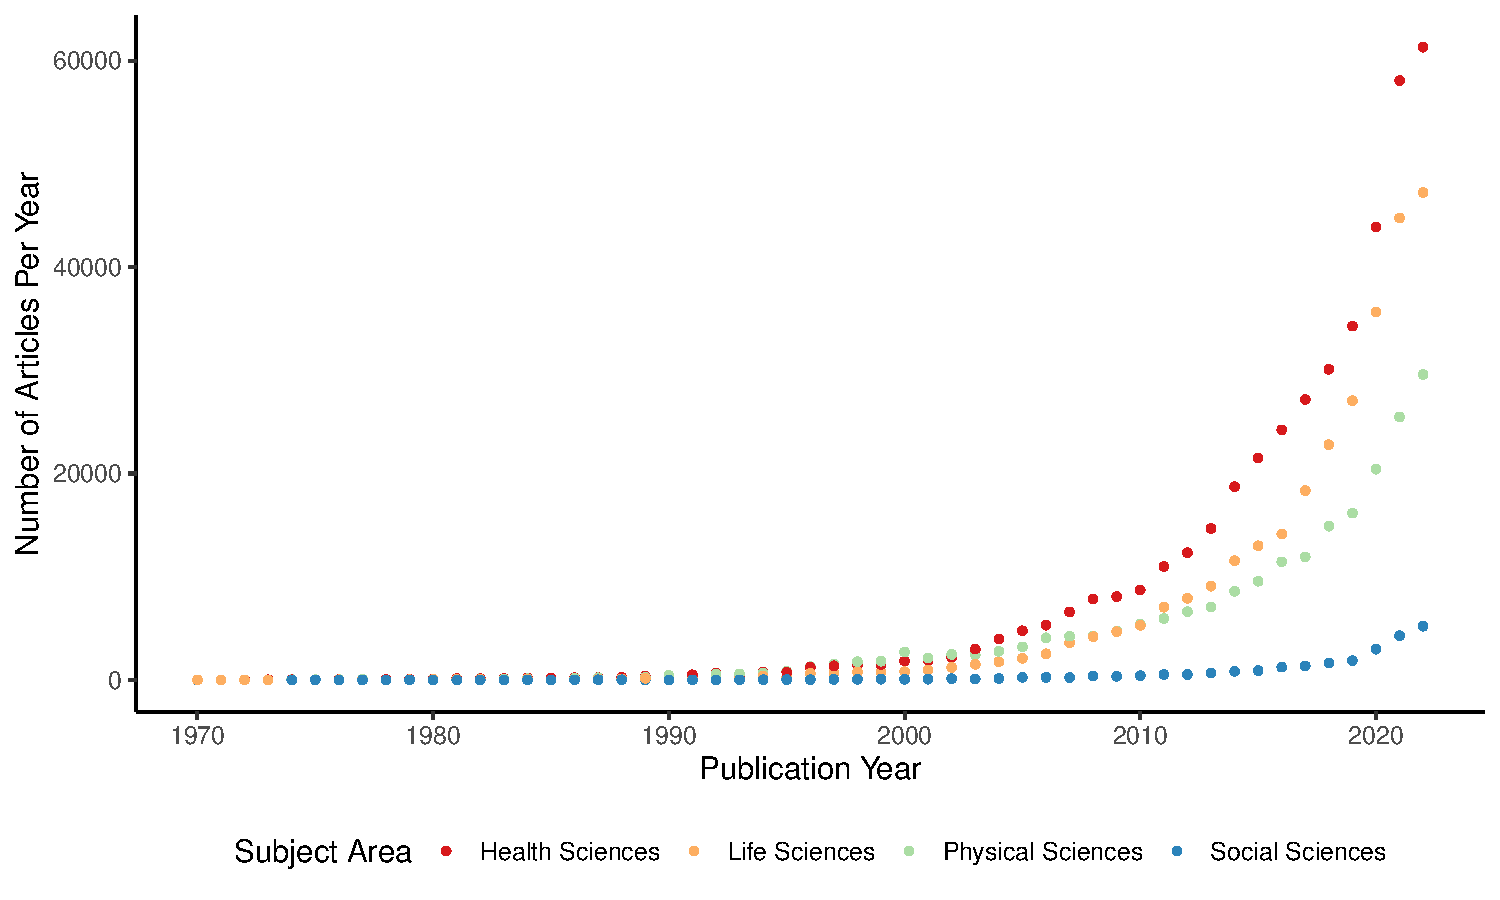
\includegraphics{manuscript_scopus_unmasked_files/figure-latex/fig-pub-time-1.pdf}
\caption{\label{fig:fig-pub-time}Number of big-team science publications separated by four large subject areas across years. All four subject areas show an exponential number of publications in the last decade.}
\end{figure}

\hypertarget{number-of-journals}{%
\subsubsection{Number of Journals}\label{number-of-journals}}

The number of distinct journals big team science
articles were published in was 14924 with 6559
journals in Health Sciences, 5787 journals in Physical
Sciences, 2500 journals in Social Sciences, and
4187 journals in Life Sciences. The descriptive statistics
for the Source Normalized Impact per Paper is presented in the
supplemental materials with a comparison for all papers.

\hypertarget{rq2-publication-information.}{%
\subsection{RQ2: Publication Information.}\label{rq2-publication-information.}}

Publication interest area was summarized by the four large subject areas
creating a word cloud plot of the total number of publications within
the ASJCs. Figure \ref{fig:fig-clouds} displays that the Health
Sciences tends to publish within medicine and oncology, with a
corresponding focus of cancer research and genetics for the Life
Sciences. The Physical Sciences was mostly dominated by physics
research, chemistry, and ecology. The BTS publications in the Social
Sciences are mostly within psychology, education, and health.

\begin{figure}
\centering
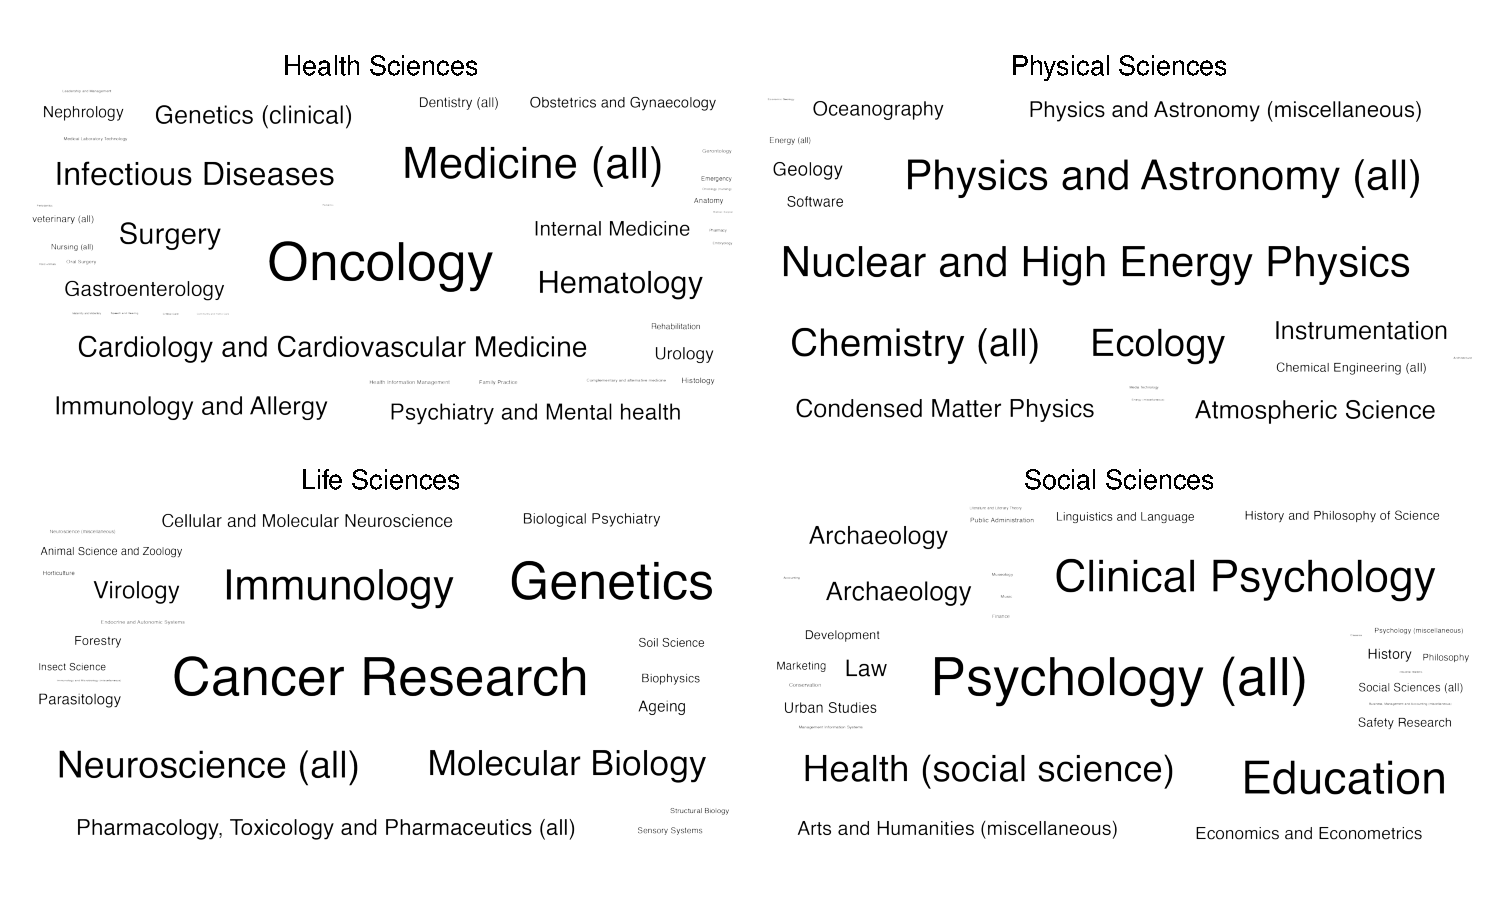
\includegraphics{manuscript_scopus_unmasked_files/figure-latex/fig-clouds-1.pdf}
\caption{\label{fig:fig-clouds}Journal Areas for Big-Team Science Publications by Subject Area. Larger words indicate more publications in those ASJC areas.}
\end{figure}

\hypertarget{rq3-author-descriptive-statistics-1}{%
\subsection{RQ3: Author Descriptive Statistics}\label{rq3-author-descriptive-statistics-1}}

The total number of unique authors across all publications was
3047067. The mean number of authors per publication was \emph{M} =
49.31 (\emph{SD} = 212.98, \emph{Med} = 18) with a
range of 10 to 5568. The median and average
number of authors by subject area are displayed in Figure
\ref{fig:fig-author-year}. In general, the average and median number of
authors increased over time, with the exception of the skew in the
Physical Sciences. Interestingly, the effect in the Physical Sciences
appears to be declining toward the general trends seen in other areas in
the last few decades.

\begin{figure}
\centering
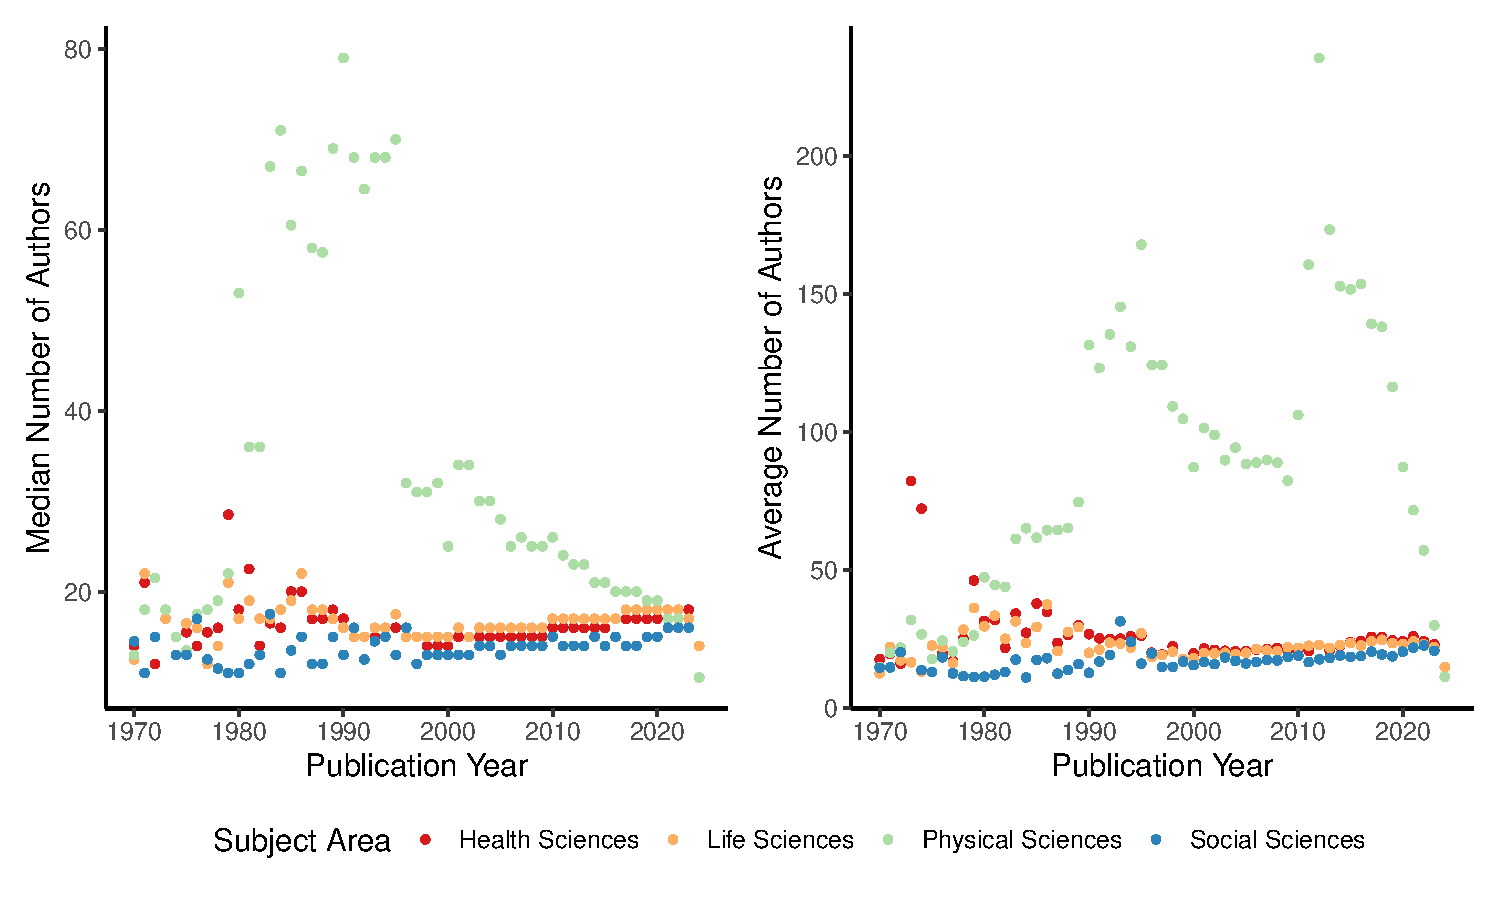
\includegraphics{manuscript_scopus_unmasked_files/figure-latex/fig-author-year-1.pdf}
\caption{\label{fig:fig-author-year}Number of authors included on big-team science papers per year by subject area. Given the large skew in the data, the left panel presents the median number of authors per manuscript, and the right panel presents the average number of authors per manuscript by year.}
\end{figure}

\hypertarget{publication-metrics-1}{%
\subsubsection{Publication Metrics}\label{publication-metrics-1}}

The average number of publications by authors on big team science papers
is \emph{M} = 38.37 (\emph{SD} = 102.54). The
publication counts were averaged across authors for each publication,
and then these average publication counts were averaged across
publications \emph{M} = 162.50 (\emph{SD} =
155.17). The average variability (i.e., the average
standard deviation with authors of a manuscript) with publication counts
of a paper was \(M_{SD}\) = 164.27 (\(SD_{SD}\) =
127.21).

The same process was completed with \emph{h}-index for each author and
publication. The average \emph{h}-index for authors overall was \emph{M} =
33.65 (\emph{SD} = 127.34, \emph{Med} = 8.00). The
average \emph{h}-index for publications was \emph{M} = 198.87 (\emph{SD}
= 248.78), and the variability of \emph{h}-index across
manuscripts was \(M_{SD}\) = 211.80 (\(SD_{SD}\) =
238.53, \(Med_{Med}\) = 68.00).

\hypertarget{institutions-1}{%
\subsubsection{Institutions}\label{institutions-1}}

The total number of unique affiliation across all papers was 463876.

\hypertarget{rq4-author-diversity-statistics-1}{%
\subsection{RQ4: Author Diversity Statistics}\label{rq4-author-diversity-statistics-1}}

\hypertarget{seniority-1}{%
\subsubsection{Seniority}\label{seniority-1}}

Figure \ref{fig:fig-career} portrays the average career length for
authors involved in BTS publications across years. Career length was
defined as the year of first publication minus the current year, and
higher numbers mean longer careers. To analyze trends over time, we
calculated the average career length for each publication (i.e., average
author career lengths to create one score for each paper) and analyzed a
regression analysis using career length to predict year of publication.
In order to show variance between individuals, we calculated the
standard deviation of career length for each publication and used this
variance as an additional predictor.

Negative career length slopes would indicate more young scholars in
later years (i.e., lower average career length as time increases).
Positive career length slopes would indicate older scholars in later
years (i.e., higher average career length as time increases). Negative
career variance slopes imply that variability decreases over the years,
so the average career length is more homogeneous. Positive career length
slopes imply that variability increases over the years, so the average
career length is varied across individuals (i.e., different stages of
scholars). Figure \ref{fig:fig-heatmap} displays the results for all
regression analyses to compare coefficient strength across and within
each hypothesis.

All values for these analyses were different from zero. The slopes for
the average career length were negative for all four subject areas,
indicating a trend toward younger scientist involvement over time for
each area, with the strongest effect in the Physical Sciences. The
coefficient for variability in career length was also negative for each
of the four subject areas with the highest in the Physical Sciences and
lowest in the Life Sciences. This result indicates a decrease in the
variability of career lengths over time, likely from two sources: 1)
more publications with more authors, thus, lowering variance
estimations, and 2) more young scholars overall. The effect sizes for
this analysis were surprisingly large ranging from \(R^2\) = .25 to .47.
All values and their confidence intervals can be found on our OSF page.

\begin{figure}
\centering
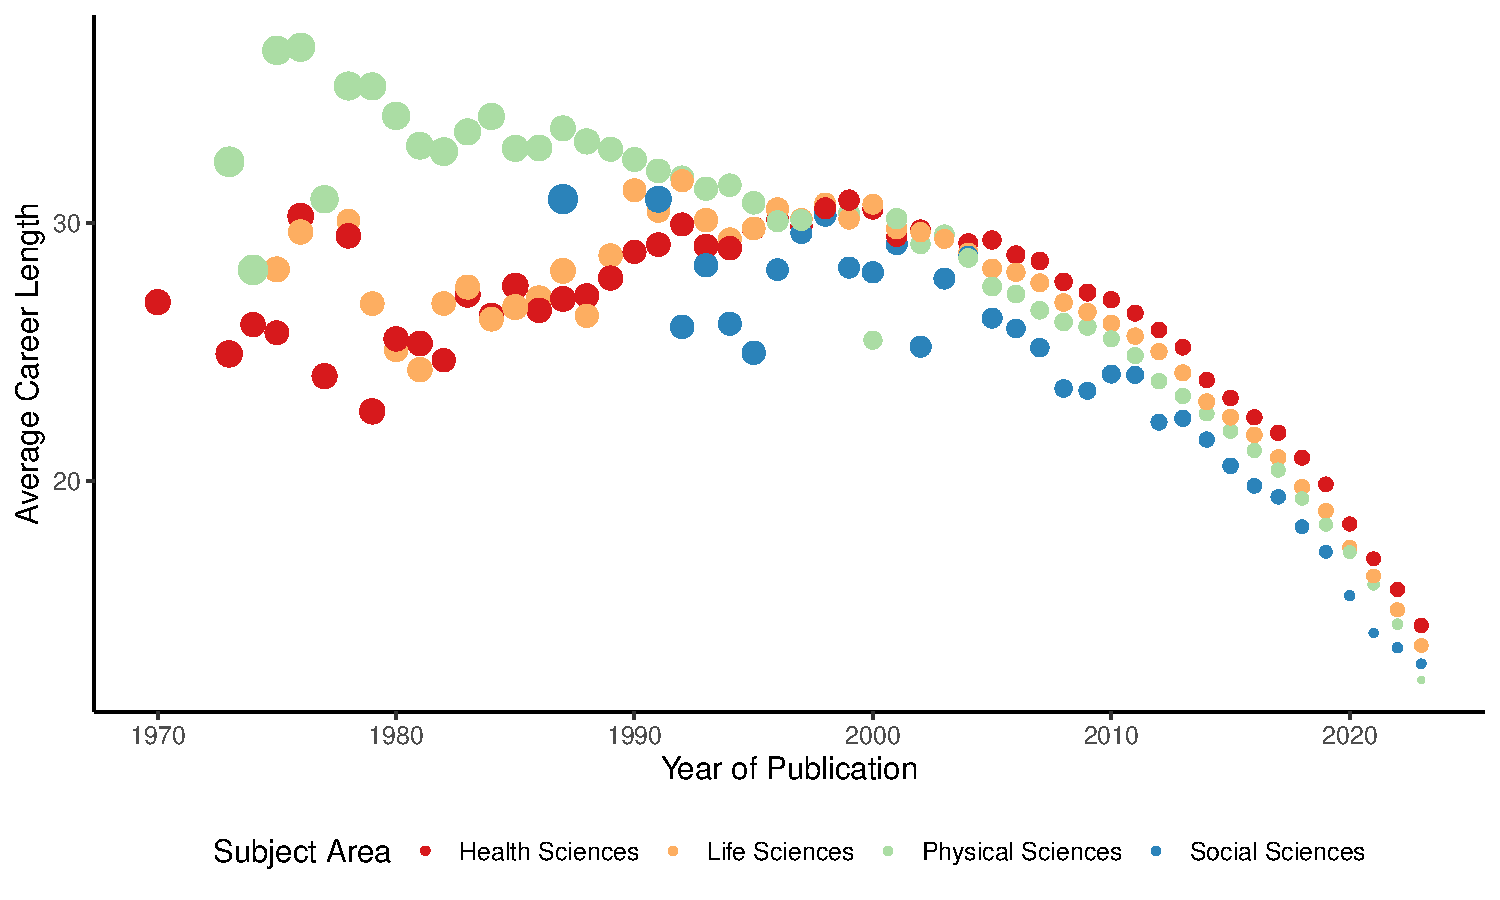
\includegraphics{manuscript_scopus_unmasked_files/figure-latex/fig-career-1.pdf}
\caption{\label{fig:fig-career}Average career length for big-team science authors. Larger dots indicate more variability in career length for authors by averaging the standard deviation in career length for each manuscript within a year. The data has been filtered to at least 10 publications in a year for this graph.}
\end{figure}

\begin{figure}
\centering
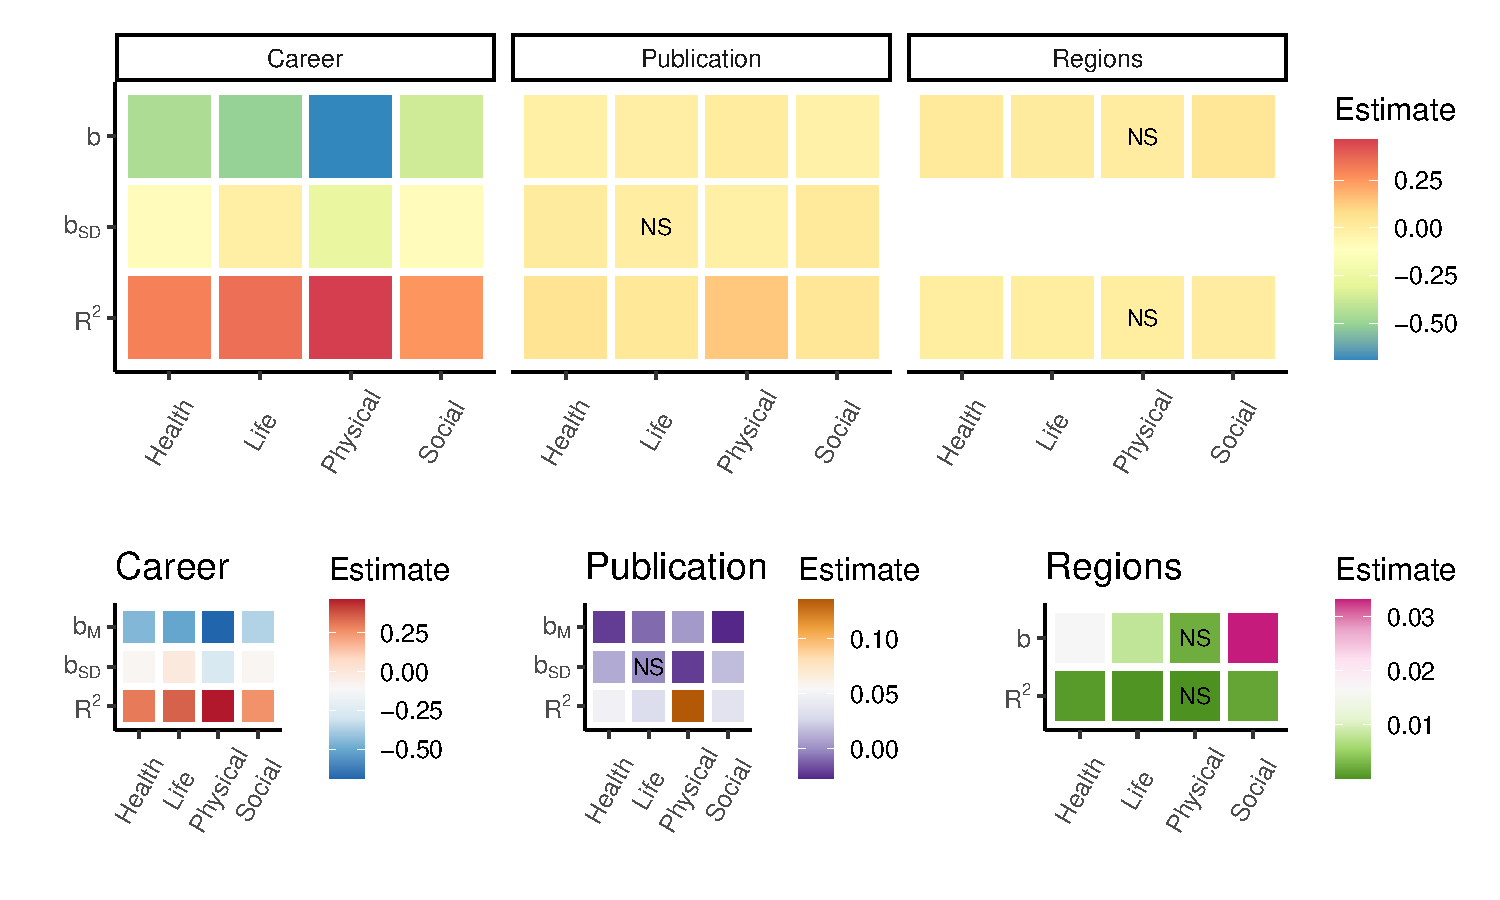
\includegraphics{manuscript_scopus_unmasked_files/figure-latex/fig-heatmap-1.pdf}
\caption{\label{fig:fig-heatmap}Heatmap results of regression analyses for career length, number of publications, and geopolitical diversity within the region. Each square represents a \emph{b} value or the slope of the predictor (x-axis) onto the dependent variable (each panel), with the exception of the bottom row which is the effect size of each regression analysis \(R^2\). Slopes included both the overall value of the predictor (\(b\), \(b_M\)) and the standard deviation of the predictor over time (\(b_{SD}\)). The color of the square represents the strength of the predictor. The top figure represents all results together for comparison across analyses. The bottom row represents individual heatmaps for each hypothesis to distinguish small differences between subject areas for those research questions. Non-significant results are indicated with NS on the plot.}
\end{figure}

We used the same analyses using number of publications to represent diversity instead of career length. An increasing slope over time indicates that
individuals who are publishing more are more represented in BTS over
time (i.e., increasing numbers of scholars with higher publication
rates), while a negative slope indicates more researchers with less
publications. A positive slope for the standard deviation of publication
metrics indicates increasing variance over time (i.e., more diversity in
the individual publication rates), while a negative slope would indicate
less diversity in researchers over time. While publication rates do not
represent value as a researcher, they are often used in hiring and
promotion decisions, and we used this variable as a proxy to gauge the
diversity in scholars represented in big teams. As shown in Figure
\ref{fig:fig-heatmap} publication metrics were generally negative for
the average publication metrics, indicating more scholars over time with
lower numbers of publications with the strongest effects in Health and
Social Sciences. The variability of publication counts was not
significant for the Life Sciences but was negative for the Physical
Sciences (less variability over time) and positive for Social and Health
Sciences (more variability and over time). This result indicates that
the Physical Sciences are trending toward scholars with less
publications but also less diverse in number of publications, while the
Health and Social Sciences see more diversity in publication counts and
less published scholars overall.

\begin{figure}
\centering
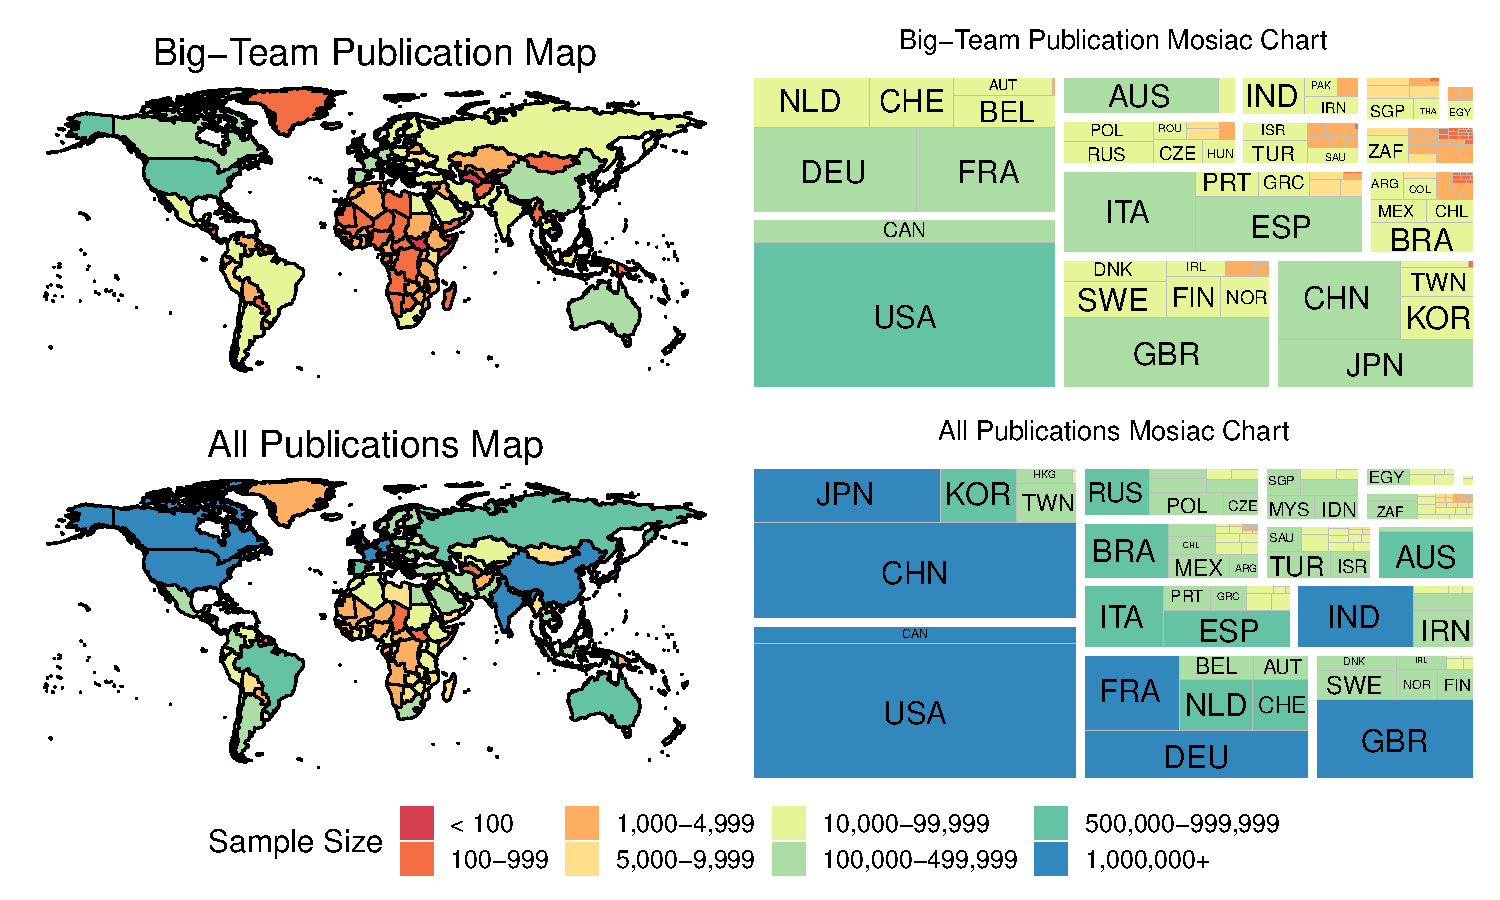
\includegraphics{manuscript_scopus_unmasked_files/figure-latex/fig-map-both-1.pdf}
\caption{\label{fig:fig-map-both}Geopolitical regions represented in big-team science publications versus all publications. The mosaic plot is grouped by UN subregion with the largest number of publications starting on the bottom left and smallest on the top right. Therefore, North America represents the largest number of authors within BTS (i.e., bottom right, then separated into the geopolitical areas within that subregion), followed by Eastern Europe (top left), and so on.}
\end{figure}

\hypertarget{geopolitical-regions}{%
\subsubsection{Geopolitical Regions}\label{geopolitical-regions}}

Author geopolitical region is displayed in Figure
\ref{fig:fig-map-both}. Big team publications appear to be led by North
America and Western Europe, while all publications are led by North
America and East Asia. To understand the change in representation
diversity, we examined if the number of regions in a publication is
predicted by the year of publication. Increasing diversity would be
represented by a positive slope, while decreasing diversity would be
represented by a negative slope. As shown in Figure
\ref{fig:fig-heatmap}, the Physical Sciences do not show a trend of
change in representation, while all other sciences showed a positive
effect increasing in the number of geopolitical regions authors
represent on publications.

Last, we examined the differences in representation for corresponding
author sets versus all other authors. For papers with 10 to 49 authors,
we used the three first authors and the last author to compare against
other authors. For 50 to 99 authors, five first authors plus last were
used, and for all papers with more than 100 authors, we used ten first
authors and the last author as the corresponding author set. We then
calculated the frequencies of each of the UN Sub-Regions for
corresponding authors versus all other authors, converting these values
to proportions. Given the expected small sample sizes of these
contingency tables, we grouped together titles based on the year of
publication. For each grouping, we then calculated the effect size of
the differences in frequencies comparing corresponding authors to all
other authors. Since this data is categorical, we used Cramer's \emph{V} to
represent the effect size. If the effect size includes zero in its
confidence interval (to four decimal places), this result will imply
that first and all other authors represent the same pattern of UN
Sub-Region diversity. Any confidence interval that does include zero
represents a difference in diversity.

\begin{figure}
\centering
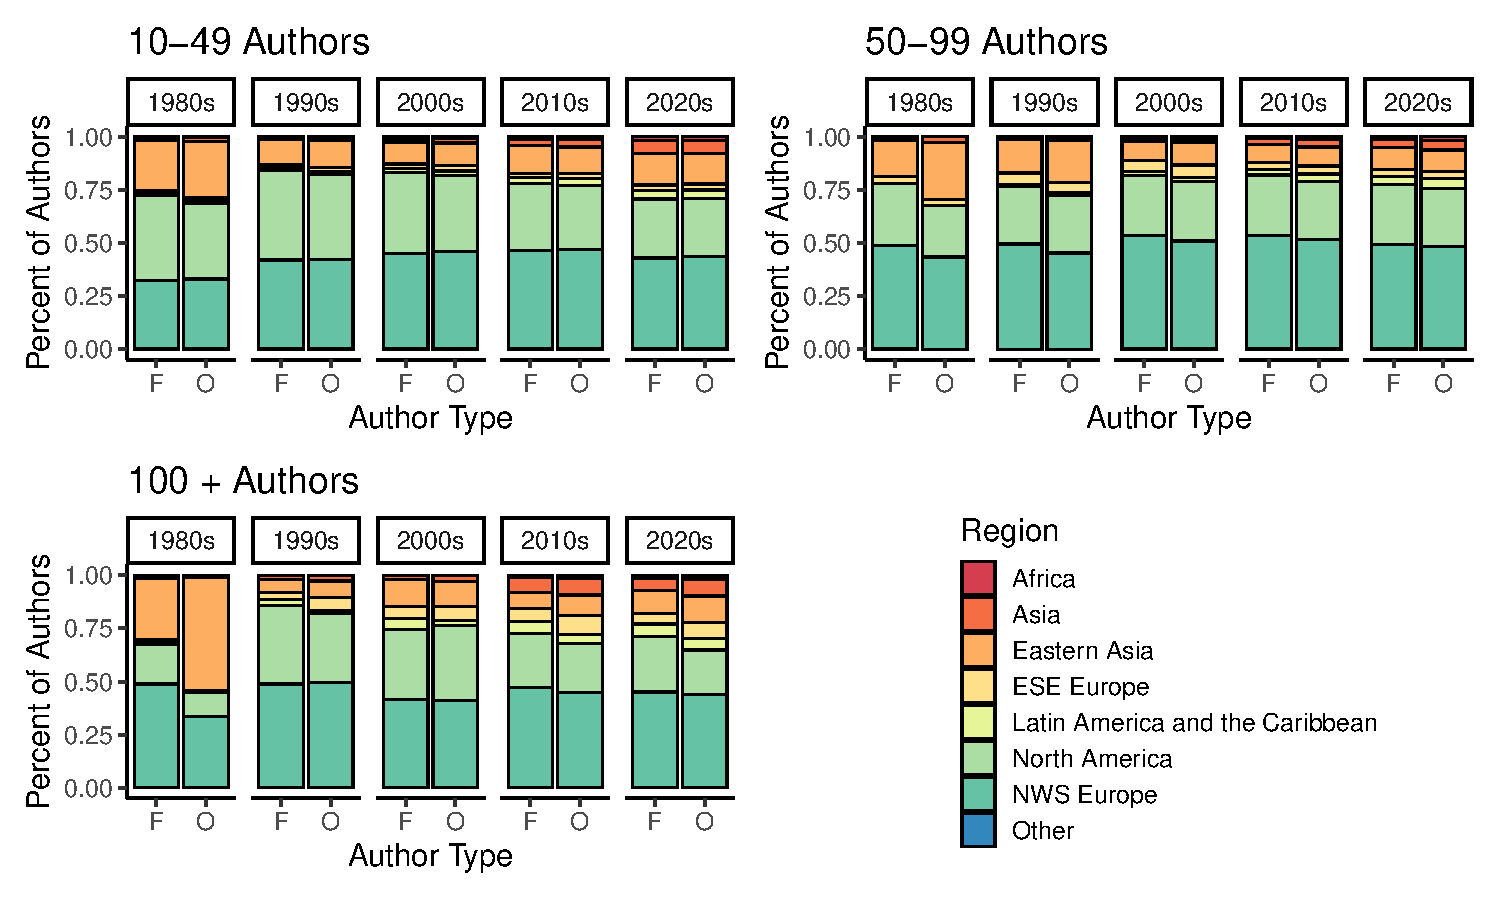
\includegraphics{manuscript_scopus_unmasked_files/figure-latex/fig-author-gpe-1.pdf}
\caption{\label{fig:fig-author-gpe}A comparison of author affiliation geopolitical regions across decades. F stands for first authors and O stands for other authors.}
\end{figure}

\begin{figure}
\centering
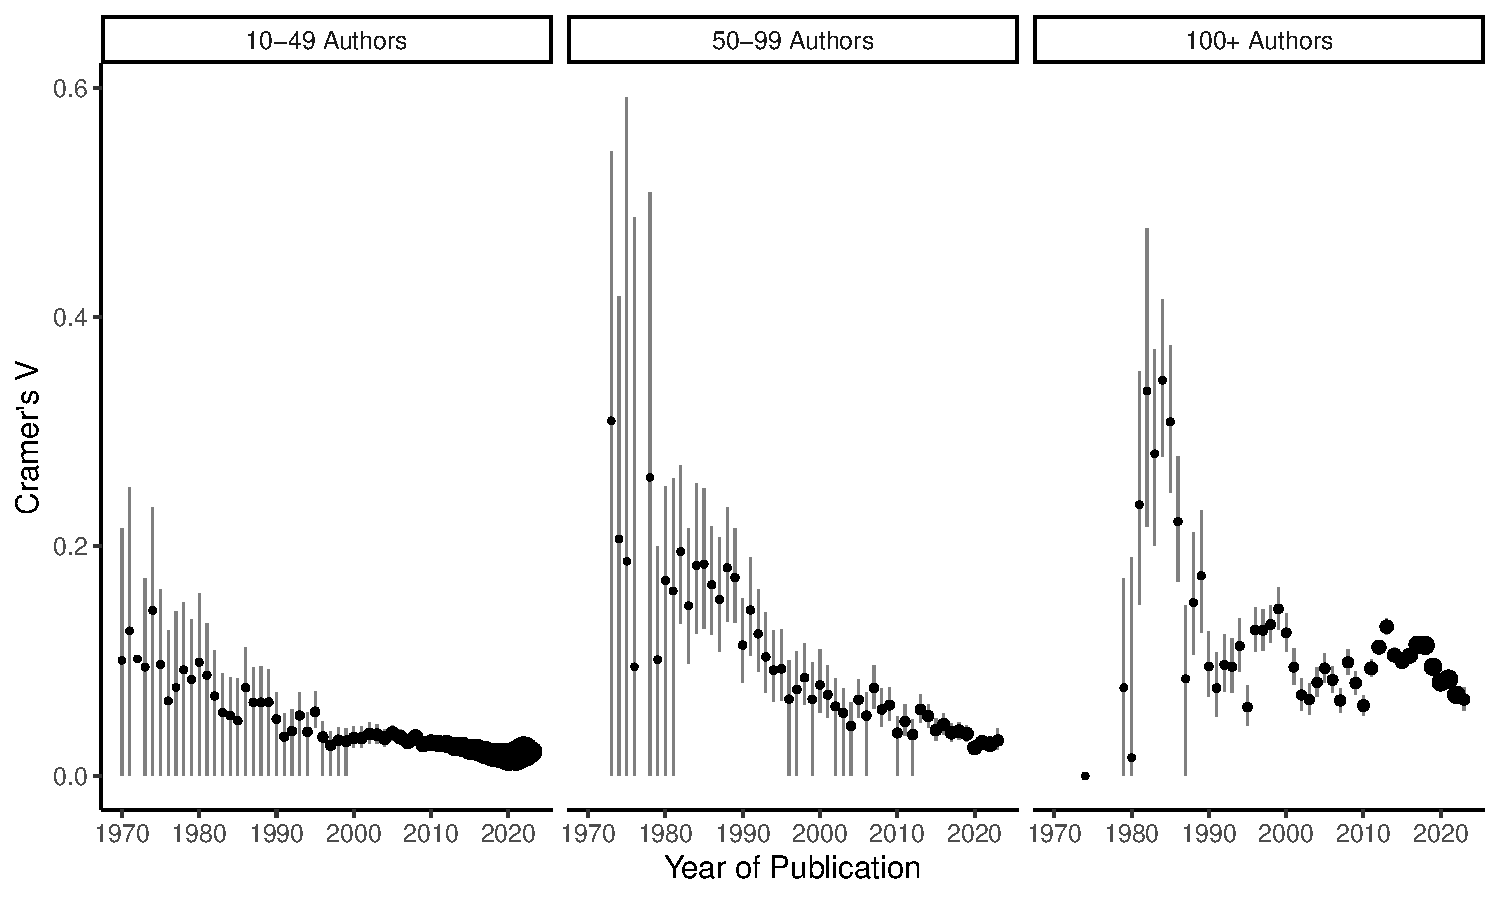
\includegraphics{manuscript_scopus_unmasked_files/figure-latex/fig-effect-gpe-1.pdf}
\caption{\label{fig:fig-effect-gpe}Effect size of the differences in representation for UN Regions for author affiliations in big-team science papers by year. Larger dots indicate more papers and authors represented in the calculation of effect size.}
\end{figure}

Figure \ref{fig:fig-author-gpe} indicates the percent of authors in
regions. In general, we found the same pattern as the overall analysis
wherein most authors are from Europe and North America. The pattern of
representation is roughly similar for the separation of small, medium,
and large numbers of authors on papers. Across time, the representation
does appear to diversify, with more representation in Asia, Latin
American, and Africa. Figure \ref{fig:fig-effect-gpe} represents the
size of the differences in first/corresponding authors and other authors
across time and number of authors. The differences in representation are
larger for papers with more authors; however, the effects are non-zero
for many of the comparisons. Encouragingly, over time these effects
appear to diminish in size. One limitation with the calculation of
effect sizes for count data is the sensitivity of the data to sample
size (i.e., \(\chi^2\) is upwardly biased by sample size, and \(V\) is
calculated based on this value). While we used the inclusion of zero as
our boundary for ``significance'', the interpretation of the effects is
that most are likely small: \(V\) \textless{} .05:
31.79\%, \(V\) \textless{} .10:
70.20\%, \(V\) \textless{}
.20: 94.04\%.

\newpage

\hypertarget{discussion}{%
\section{Discussion}\label{discussion}}

In this investigation, we explored the publication rates, areas, and researchers involved in BTS publications. Over a half-million articles were published in nearly 15,000 journals since 1970 that qualified as BTS articles. The areas of publication were aligned to cancer and genetics research in medicine and oncology for Health and Life Sciences, physics and chemistry for the Physical Sciences, and psychology for the Social Sciences. All areas of research show growth in the number of publications and authors included on manuscripts, replicating previous investigations (Hunter \& Leahey, 2008; Sinatra et al., 2015; Wuchty et al., 2007).

Our investigation expands previous research by additionally focusing on diversity in seniority of authors and geopolitical affiliation. The number of earlier career scholars increased across years, indicating that big teams may be accessible to different types of individuals, not just older, established researchers. This result is especially interesting given the publish-or-perish model still present in most institutions, as it may seem that large-scale projects could be a risky choice for non-permanent researchers. BTS projects are often slow to publish, there is no guarantee for publication, and incentives are often lower for non-corresponding authors. However, with a large team, the distribution of work could imply less effort on individual non-leading members, and research has shown that larger-team publications do receive more citations and appear to have higher impact (Larivière et al., 2015).

In general, it appears that there is a decrease in the average number of publications a researcher has when publishing in a BTS paper over time, mirroring career length results. This result is likely attributable to the number of early career scholars joining projects, but also may support increased accessibility for individuals to be involved. Globalization, the internet, and the focus on interdisciplinary research are potentially driving forces behind our results, but, hopefully, the results also point to a decline in scientific gatekeeping (Lu, 2007; Siler et al., 2015).

The variability in the types of researchers involved in publications
also decreased across time in most areas of science with a decrease in
variability for career length. As mentioned, an increase in early career
researchers and numbers of publications could explain this effect
mathematically, potentially with other social influences mentioned
above. The variability in the number of publications is decreasing in
the Physical Sciences, mirroring the career length results, but the
opposite effect was found in the Health and Social Sciences. We see no
clear reason why career variability would decrease while the variability
in the number of publications would increase. The effect sizes for
career length were much larger than the effects for number of
publications. One speculation is the increasing requirements for a
competitive faculty role application. Given the limited number of
positions, one potential way to distinguish their application would be a
larger number of publications in their early career (Caplow, 2017; Kyvik, 2003).

The number of geopolitical entities for researcher affiliation is
increasing over time, showing the results of globalization and the
ability to connect across time zones and cultures (Xie, 2014). While our
definition of BTS required at least ten different
institutional affiliations, we did not filter papers by geopolitical
region, and thus, a manuscript could rely solely on institutions within
a single country. The Physical Sciences did not show an increase in
diversity of regions represented, however, it could be argued that the
development of large research centers like CERN forced earlier diversity
than other sciences (i.e., because CERN specifically recruited
scientists from sponsoring nations). The Life, Health, and Social
Sciences saw an increase in the number of regions represented with the
highest increase in the Social Sciences. This result likely corresponds
with an increased interest in big team science publications in
psychology (Coles et al., 2022; Forscher et al., 2022), and the desire to diversify the
populations represented in psychological research (Henrich et al., 2010; Newson et al., 2021).

While publications overall are diversifying, we found differences in the representation for first/corresponding authors versus all other authors. In general, first authors appear to be less diverse, representing European and North American authors, while other authors include more Asian and African authors. These effect sizes were often small, but the inequality persists across years. Diverse teams are more likely to have papers with stronger ``impact'' (Freeman \& Huang, 2015; Hinnant et al., 2012; B. F. Jones et al., 2008; Yang et al., 2022) with higher citation metrics for more diverse author lists.
The introduction of contributorship models (e.g., CRediT, Allen et al., 2019)
will hopefully continue to push these effects down, as they highlight
each individual's contribution to a manuscript.

The limitations for this research are tied to the curation of the Scopus dataset: the correct author affiliations, the correct author publication information, and the correctly marked geopolitical entity. We had planned to analyze educational levels change over time; however, this data was mostly blank within the Scopus archive. Scopus is a carefully curated and large dataset, but these limitations must be kept in mind when interpreting the results. Publication language diversity was not investigated, and a previous study indicates that most publications in big databases are in English (Albarillo, 2014). Certainly, publications in non-English
languages would improve the statistics on diversity in scientific
publishing - but the English language barrier likely exists regardless
of inclusion in databases (Meneghini \& Packer, 2007; Ramírez-Castañeda, 2020).

Big teams can provide high-impact, important research within scientific publishing, and this report suggests a promising trend of increasing publications that include earlier career and more diverse scholars. These partnerships introduce new challenges to collaboration from interpersonal conflict, infrastructure, incentives, to international political situations (Forscher et al., 2022). The implications for retention and promotion processes across a broad span of regions should be explored to improve diversity with the understanding of the differential impact of incentives for participating in big team studies.

\newpage

\hypertarget{references}{%
\section{References}\label{references}}

\begingroup
\setlength{\parindent}{-0.5in}

\hypertarget{refs}{}
\begin{CSLReferences}{1}{0}
\leavevmode\vadjust pre{\hypertarget{ref-aphilos2021}{}}%
A philosophical case for big physics. (2021). \emph{Nature Physics}, \emph{17}(6), 661--661. \url{https://doi.org/10.1038/s41567-021-01278-0}

\leavevmode\vadjust pre{\hypertarget{ref-albarillo2014}{}}%
Albarillo, F. (2014). Language in social science databases: English versus non-english articles in JSTOR and scopus. \emph{Behavioral \& Social Sciences Librarian}, \emph{33}(2), 77--90. \url{https://doi.org/10.1080/01639269.2014.904693}

\leavevmode\vadjust pre{\hypertarget{ref-allen2019}{}}%
Allen, L., O'Connell, A., \& Kiermer, V. (2019). How can we ensure visibility and diversity in research contributions? How the Contributor Role Taxonomy (CRediT) is helping the shift from authorship to contributorship. \emph{Learned Publishing}, \emph{32}(1), 71--74. \url{https://doi.org/10.1002/leap.1210}

\leavevmode\vadjust pre{\hypertarget{ref-auspurg2021}{}}%
Auspurg, K., \& Brüderl, J. (2021). Has the Credibility of the Social Sciences Been Credibly Destroyed? Reanalyzing the {``}Many Analysts, One Data Set{''} Project. \emph{Socius: Sociological Research for a Dynamic World}, \emph{7}. \url{https://doi.org/10.1177/23780231211024421}

\leavevmode\vadjust pre{\hypertarget{ref-bago2022}{}}%
Bago, B., Kovacs, M., Protzko, J., Nagy, T., Kekecs, Z., Palfi, B., Adamkovic, M., Adamus, S., Albalooshi, S., Albayrak-Aydemir, N., Alfian, I. N., Alper, S., Alvarez-Solas, S., Alves, S. G., Amaya, S., Andresen, P. K., Anjum, G., Ansari, D., Arriaga, P., \ldots{} Aczel, B. (2022). Situational factors shape moral judgements in the trolley dilemma in Eastern, Southern and Western countries in a culturally diverse sample. \emph{Nature Human Behaviour}, \emph{6}, 880--895. \url{https://doi.org/10.1038/s41562-022-01319-5}

\leavevmode\vadjust pre{\hypertarget{ref-buchanan2023}{}}%
Buchanan, E. M., Lewis, S. C., Paris, B., Forscher, P. S., Pavlacic, J. M., Beshears, J. E., Drexler, S. M., Gourdon-Kanhukamwe, A., Mallik, P. R., Silan, M. A. A., Miller, J. K., IJzerman, H., Moshontz, H., Beaudry, J. L., Suchow, J. W., Chartier, C. R., Coles, N. A., Sharifian, M., Todsen, A. L., \ldots{} McFall, J. P. (2023). The psychological science accelerator{'}s COVID-19 rapid-response dataset. \emph{Scientific Data}, \emph{10}(1), 87. \url{https://doi.org/10.1038/s41597-022-01811-7}

\leavevmode\vadjust pre{\hypertarget{ref-buttrick2020}{}}%
Buttrick, N. R., Aczel, B., Aeschbach, L. F., Bakos, B. E., Brühlmann, F., Claypool, H. M., Hüffmeier, J., Kovacs, M., Schuepfer, K., Szecsi, P., Szuts, A., Szöke, O., Thomae, M., Torka, A.-K., Walker, R. J., \& Wood, M. J. (2020). Many Labs 5: Registered Replication of Vohs and Schooler (2008), Experiment 1. \emph{Advances in Methods and Practices in Psychological Science}, \emph{3}(3), 429--438. \url{https://doi.org/10.1177/2515245920917931}

\leavevmode\vadjust pre{\hypertarget{ref-caplow2017}{}}%
Caplow, T. (2017). \emph{The academic marketplace} (2nd ed.). Routledge. \url{https://doi.org/10.4324/9781351305969}

\leavevmode\vadjust pre{\hypertarget{ref-castelnovo2018}{}}%
Castelnovo, P., Florio, M., Forte, S., Rossi, L., \& Sirtori, E. (2018). The economic impact of technological procurement for large-scale research infrastructures: Evidence from the Large Hadron Collider at CERN. \emph{Research Policy}, \emph{47}(9), 1853--1867. \url{https://doi.org/10.1016/j.respol.2018.06.018}

\leavevmode\vadjust pre{\hypertarget{ref-coles2022}{}}%
Coles, N. A., Hamlin, J. K., Sullivan, L. L., Parker, T. H., \& Altschul, D. (2022). Build up big-team science. \emph{Nature}, \emph{601}(7894), 505--507. \url{https://doi.org/10.1038/d41586-022-00150-2}

\leavevmode\vadjust pre{\hypertarget{ref-collins2003}{}}%
Collins, F. S., Morgan, M., \& Patrinos, A. (2003). The human genome project: Lessons from large-scale biology. \emph{Science}, \emph{300}(5617), 286--290. \url{https://doi.org/10.1126/science.1084564}

\leavevmode\vadjust pre{\hypertarget{ref-dorison2022}{}}%
Dorison, C. A., Lerner, J. S., Heller, B. H., Rothman, A. J., Kawachi, I. I., Wang, K., Rees, V. W., Gill, B. P., Gibbs, N., Ebersole, C. R., Vally, Z., Tajchman, Z., Zsido, A. N., Zrimsek, M., Chen, Z., Ziano, I., Gialitaki, Z., Ceary, C. D., Lin, Y., \ldots{} Coles, N. A. (2022). In {COVID}-19 {Health} {Messaging}, {Loss} {Framing} {Increases} {Anxiety} with {Little}-to-{No} {Concomitant} {Benefits}: {Experimental} {Evidence} from 84 {Countries}. \emph{Affective Science}, \emph{3}(3), 577--602. \url{https://doi.org/10.1007/s42761-022-00128-3}

\leavevmode\vadjust pre{\hypertarget{ref-ebersole2016}{}}%
Ebersole, C. R., Atherton, O. E., Belanger, A. L., Skulborstad, H. M., Allen, J. M., Banks, J. B., Baranski, E., Bernstein, M. J., Bonfiglio, D. B. V., Boucher, L., Brown, E. R., Budiman, N. I., Cairo, A. H., Capaldi, C. A., Chartier, C. R., Chung, J. M., Cicero, D. C., Coleman, J. A., Conway, J. G., \ldots{} Nosek, B. A. (2016). Many Labs 3: Evaluating participant pool quality across the academic semester via replication. \emph{Journal of Experimental Social Psychology}, \emph{67}, 68--82. \url{https://doi.org/10.1016/j.jesp.2015.10.012}

\leavevmode\vadjust pre{\hypertarget{ref-ebersole2020}{}}%
Ebersole, C. R., Mathur, M. B., Baranski, E., Bart-Plange, D.-J., Buttrick, N. R., Chartier, C. R., Corker, K. S., Corley, M., Hartshorne, J. K., IJzerman, H., Lazarević, L. B., Rabagliati, H., Ropovik, I., Aczel, B., Aeschbach, L. F., Andrighetto, L., Arnal, J. D., Arrow, H., Babincak, P., \ldots{} Nosek, B. A. (2020). Many Labs 5: Testing Pre-Data-Collection Peer Review as an Intervention to Increase Replicability. \emph{Advances in Methods and Practices in Psychological Science}, \emph{3}(3), 309--331. \url{https://doi.org/10.1177/2515245920958687}

\leavevmode\vadjust pre{\hypertarget{ref-10.7554ux2feLife.71601}{}}%
Errington, T. M., Mathur, M., Soderberg, C. K., Denis, A., Perfito, N., Iorns, E., \& Nosek, B. A. (2021). Investigating the replicability of preclinical cancer biology. \emph{eLife}, \emph{10}, e71601. \url{https://doi.org/10.7554/eLife.71601}

\leavevmode\vadjust pre{\hypertarget{ref-forscher2022a}{}}%
Forscher, P. S., Wagenmakers, E.-J., Coles, N. A., Silan, M. A., Dutra, N., Basnight-Brown, D., \& IJzerman, H. (2022). The Benefits, Barriers, and Risks of Big-Team Science. \emph{Perspectives on Psychological Science}, \emph{18}(3), 607623. \url{https://doi.org/10.1177/17456916221082970}

\leavevmode\vadjust pre{\hypertarget{ref-franco2014}{}}%
Franco, A., Malhotra, N., \& Simonovits, G. (2014). Publication bias in the social sciences: Unlocking the file drawer. \emph{Science}, \emph{345}(6203), 1502--1505. \url{https://doi.org/10.1126/science.1255484}

\leavevmode\vadjust pre{\hypertarget{ref-freeman2015}{}}%
Freeman, R. B., \& Huang, W. (2015). Collaborating with People Like Me: Ethnic Coauthorship within the United States. \emph{Journal of Labor Economics}, \emph{33}(S1), S289--S318. \url{https://doi.org/10.1086/678973}

\leavevmode\vadjust pre{\hypertarget{ref-grahe2014}{}}%
Grahe, J. E. (2014). Announcing open science badges and reaching for the sky. \emph{The Journal of Social Psychology}, \emph{154}(1), 1--3. \url{https://doi.org/10.1080/00224545.2014.853582}

\leavevmode\vadjust pre{\hypertarget{ref-henrich2010}{}}%
Henrich, J., Heine, S. J., \& Norenzayan, A. (2010). The weirdest people in the world? \emph{Behavioral and Brain Sciences}, \emph{33}(2-3), 61--83. \url{https://doi.org/10.1017/S0140525X0999152X}

\leavevmode\vadjust pre{\hypertarget{ref-hinnant2012}{}}%
Hinnant, C. C., Stvilia, B., Wu, S., Worrall, A., Burnett, G., Burnett, K., Kazmer, M. M., \& Marty, P. F. (2012). Author-team diversity and the impact of scientific publications: Evidence from physics research at a national science lab. \emph{Library \& Information Science Research}, \emph{34}(4), 249--257. \url{https://doi.org/10.1016/j.lisr.2012.03.001}

\leavevmode\vadjust pre{\hypertarget{ref-hubbard1997}{}}%
Hubbard, R., \& Armstrong, J. S. (1997). Publication Bias against Null Results. \emph{Psychological Reports}, \emph{80}(1), 337--338. \url{https://doi.org/10.2466/pr0.1997.80.1.337}

\leavevmode\vadjust pre{\hypertarget{ref-hunter2008}{}}%
Hunter, L., \& Leahey, E. (2008). Collaborative Research in Sociology: Trends and Contributing Factors. \emph{The American Sociologist}, \emph{39}(4), 290--306. \url{https://doi.org/10.1007/s12108-008-9042-1}

\leavevmode\vadjust pre{\hypertarget{ref-isager2021a}{}}%
Isager, P. M., Van Aert, R. C. M., Bahník, Š., Brandt, M. J., DeSoto, K. A., Giner-Sorolla, R., Krueger, J. I., Perugini, M., Ropovik, I., Van 'T Veer, A. E., Vranka, M., \& Lakens, D. (2023). Deciding what to replicate: {A} decision model for replication study selection under resource and knowledge constraints. \emph{Psychological Methods}, \emph{28}(2), 438--451. \url{https://doi.org/10.1037/met0000438}

\leavevmode\vadjust pre{\hypertarget{ref-isager2021}{}}%
Isager, P. M., van 't Veer, A. E., \& Lakens, D. (2021). \emph{Replication value as a function of citation impact and sample size}. \url{https://doi.org/10.31222/osf.io/knjea}

\leavevmode\vadjust pre{\hypertarget{ref-john2012}{}}%
John, L. K., Loewenstein, G., \& Prelec, D. (2012). Measuring the Prevalence of Questionable Research Practices With Incentives for Truth Telling. \emph{Psychological Science}, \emph{23}(5), 524--532. \url{https://doi.org/10.1177/0956797611430953}

\leavevmode\vadjust pre{\hypertarget{ref-jones2021}{}}%
Jones, B. C., DeBruine, L. M., Flake, J. K., Liuzza, M. T., Antfolk, J., Arinze, N. C., Ndukaihe, I. L. G., Bloxsom, N. G., Lewis, S. C., Foroni, F., Willis, M. L., Cubillas, C. P., Vadillo, M. A., Turiegano, E., Gilead, M., Simchon, A., Saribay, S. A., Owsley, N. C., Jang, C., \ldots{} Coles, N. A. (2021). To which world regions does the valence{\textendash}dominance model of social perception apply? \emph{Nature Human Behaviour}, \emph{5}(1), 159--169. \url{https://doi.org/10.1038/s41562-020-01007-2}

\leavevmode\vadjust pre{\hypertarget{ref-jones2008}{}}%
Jones, B. F., Wuchty, S., \& Uzzi, B. (2008). Multi-university research teams: Shifting impact, geography, and stratification in science. \emph{Science}, \emph{322}(5905), 1259--1262. \url{https://doi.org/10.1126/science.1158357}

\leavevmode\vadjust pre{\hypertarget{ref-kidwell2016}{}}%
Kidwell, M. C., Lazarević, L. B., Baranski, E., Hardwicke, T. E., Piechowski, S., Falkenberg, L.-S., Kennett, C., Slowik, A., Sonnleitner, C., Hess-Holden, C., Errington, T. M., Fiedler, S., \& Nosek, B. A. (2016). Badges to Acknowledge Open Practices: A Simple, Low-Cost, Effective Method for Increasing Transparency. \emph{PLOS Biology}, \emph{14}(5), e1002456. \url{https://doi.org/10.1371/journal.pbio.1002456}

\leavevmode\vadjust pre{\hypertarget{ref-klein2022}{}}%
Klein, R. A., Cook, C. L., Ebersole, C. R., Vitiello, C., Nosek, B. A., Hilgard, J., Ahn, P. H., Brady, A. J., Chartier, C. R., Christopherson, C. D., Clay, S., Collisson, B., Crawford, J. T., Cromar, R., Gardiner, G., Gosnell, C. L., Grahe, J., Hall, C., Howard, I., \ldots{} Ratliff, K. A. (2022). Many Labs 4: Failure to Replicate Mortality Salience Effect With and Without Original Author Involvement. \emph{Collabra: Psychology}, \emph{8}(1), 35271. \url{https://doi.org/10.1525/collabra.35271}

\leavevmode\vadjust pre{\hypertarget{ref-klein2018}{}}%
Klein, R. A., Vianello, M., Hasselman, F., Adams, B. G., Adams, R. B., Alper, S., Aveyard, M., Axt, J. R., Babalola, M. T., Bahník, Š., Batra, R., Berkics, M., Bernstein, M. J., Berry, D. R., Bialobrzeska, O., Binan, E. D., Bocian, K., Brandt, M. J., Busching, R., \ldots{} Nosek, B. A. (2018). Many Labs 2: Investigating Variation in Replicability Across Samples and Settings. \emph{Advances in Methods and Practices in Psychological Science}, \emph{1}(4), 443--490. \url{https://doi.org/10.1177/2515245918810225}

\leavevmode\vadjust pre{\hypertarget{ref-kyvik2003}{}}%
Kyvik, S. (2003). Changing trends in publishing behaviour among university faculty, 1980-2000. \emph{Scientometrics}, \emph{58}(1), 35--48. \url{https://doi.org/10.1023/A:1025475423482}

\leavevmode\vadjust pre{\hypertarget{ref-lariviuxe8re2015}{}}%
Larivière, V., Gingras, Y., Sugimoto, C. R., \& Tsou, A. (2015). Team size matters: Collaboration and scientific impact since 1900. \emph{Journal of the Association for Information Science and Technology}, \emph{66}(7), 1323--1332. \url{https://doi.org/10.1002/asi.23266}

\leavevmode\vadjust pre{\hypertarget{ref-lebel2018}{}}%
LeBel, E. P., McCarthy, R. J., Earp, B. D., Elson, M., \& Vanpaemel, W. (2018). A Unified Framework to Quantify the Credibility of Scientific Findings. \emph{Advances in Methods and Practices in Psychological Science}, \emph{1}(3), 389--402. \url{https://doi.org/10.1177/2515245918787489}

\leavevmode\vadjust pre{\hypertarget{ref-lu2007}{}}%
Lu, Y. (2007). The human in human information acquisition: Understanding gatekeeping and proposing new directions in scholarship. \emph{Library \& Information Science Research}, \emph{29}(1), 103--123. \url{https://doi.org/10.1016/j.lisr.2006.10.007}

\leavevmode\vadjust pre{\hypertarget{ref-maizey2019}{}}%
Maizey, L., \& Tzavella, L. (2019). Barriers and solutions for early career researchers in tackling the reproducibility crisis in cognitive neuroscience. \emph{Cortex}, \emph{113}, 357--359. \url{https://doi.org/10.1016/j.cortex.2018.12.015}

\leavevmode\vadjust pre{\hypertarget{ref-mathur2020}{}}%
Mathur, M. B., Bart-Plange, D.-J., Aczel, B., Bernstein, M. H., Ciunci, A. M., Ebersole, C. R., Falcão, F., Ashbaugh, K., Hilliard, R. A., Jern, A., Kellier, D. J., Kessinger, G., Kolb, V. S., Kovacs, M., Lage, C. A., Langford, E. V., Lins, S., Manfredi, D., Meyet, V., \ldots{} Frank, M. C. (2020). Many Labs 5: Registered Multisite Replication of the Tempting-Fate Effects in Risen and Gilovich (2008). \emph{Advances in Methods and Practices in Psychological Science}, \emph{3}(3), 394--404. \url{https://doi.org/10.1177/2515245918785165}

\leavevmode\vadjust pre{\hypertarget{ref-maxwell2015}{}}%
Maxwell, S. E., Lau, M. Y., \& Howard, G. S. (2015). Is psychology suffering from a replication crisis?: What does 'failure to replicate' really mean? \emph{American Psychologist}, \emph{70}(6), 487--498. \url{https://doi.org/10.1037/a0039400}

\leavevmode\vadjust pre{\hypertarget{ref-mayo-wilson2021}{}}%
Mayo-Wilson, E., Grant, S., Supplee, L., Kianersi, S., Amin, A., DeHaven, A., \& Mellor, D. (2021). Evaluating implementation of the transparency and openness promotion~(TOP) guidelines:~The TRUST process for rating journal policies, procedures, and practices. \emph{Research Integrity and Peer Review}, \emph{6}(1), 9. \url{https://doi.org/10.1186/s41073-021-00112-8}

\leavevmode\vadjust pre{\hypertarget{ref-meneghini2007}{}}%
Meneghini, R., \& Packer, A. L. (2007). Is there science beyond english? \emph{EMBO Reports}, \emph{8}(2), 112--116. \url{https://doi.org/10.1038/sj.embor.7400906}

\leavevmode\vadjust pre{\hypertarget{ref-moshontz2018}{}}%
Moshontz, H., Campbell, L., Ebersole, C. R., IJzerman, H., Urry, H. L., Forscher, P. S., Grahe, J. E., McCarthy, R. J., Musser, E. D., Antfolk, J., Castille, C. M., Evans, T. R., Fiedler, S., Flake, J. K., Forero, D. A., Janssen, S. M. J., Keene, J. R., Protzko, J., Aczel, B., \ldots{} Chartier, C. R. (2018). The Psychological Science Accelerator: Advancing Psychology Through a Distributed Collaborative Network. \emph{Advances in Methods and Practices in Psychological Science}, \emph{1}(4), 501--515. \url{https://doi.org/10.1177/2515245918797607}

\leavevmode\vadjust pre{\hypertarget{ref-nelson2018}{}}%
Nelson, L. D., Simmons, J., \& Simonsohn, U. (2018). Psychology's renaissance. \emph{Annual Review of Psychology}, \emph{69}(1), 511--534. \url{https://doi.org/10.1146/annurev-psych-122216-011836}

\leavevmode\vadjust pre{\hypertarget{ref-newson2021}{}}%
Newson, M., Buhrmester, M., Xygalatas, D., \& Whitehouse, H. (2021). Go WILD, not WEIRD. \emph{Journal for the Cognitive Science of Religion}, \emph{6}(1-2). \url{https://doi.org/10.1558/jcsr.38413}

\leavevmode\vadjust pre{\hypertarget{ref-nosek2015}{}}%
Nosek, B. A., Alter, G., Banks, G. C., Borsboom, D., Bowman, S. D., Breckler, S. J., Buck, S., Chambers, C. D., Chin, G., Christensen, G., Contestabile, M., Dafoe, A., Eich, E., Freese, J., Glennerster, R., Goroff, D., Green, D. P., Hesse, B., Humphreys, M., \ldots{} Yarkoni, T. (2015). Promoting an open research culture. \emph{Science}, \emph{348}(6242), 1422--1425. \url{https://doi.org/10.1126/science.aab2374}

\leavevmode\vadjust pre{\hypertarget{ref-nosek2014method}{}}%
Nosek, B. A., \& Lakens, D. (2014a). A method to increase the credibility of published results. \emph{Social Psychology}, \emph{45}(3), 137141.

\leavevmode\vadjust pre{\hypertarget{ref-nosek2014}{}}%
Nosek, B. A., \& Lakens, D. (2014b). Registered Reports: A Method to Increase the Credibility of Published Results. \emph{Social Psychology}, \emph{45}(3), 137--141. \url{https://doi.org/10.1027/1864-9335/a000192}

\leavevmode\vadjust pre{\hypertarget{ref-nosek2012}{}}%
Nosek, B. A., Spies, J. R., \& Motyl, M. (2012). Scientific Utopia: II. Restructuring Incentives and Practices to Promote Truth Over Publishability. \emph{Perspectives on Psychological Science}, \emph{7}(6), 615--631. \url{https://doi.org/10.1177/1745691612459058}

\leavevmode\vadjust pre{\hypertarget{ref-opensciencecollaboration2015}{}}%
Open Science Collaboration. (2015). Estimating the reproducibility of psychological science. \emph{Science}, \emph{349}(6251), aac4716--aac4716. \url{https://doi.org/10.1126/science.aac4716}

\leavevmode\vadjust pre{\hypertarget{ref-psychologicalscienceacceleratorself-determinationtheorycollaboration2022}{}}%
Psychological Science Accelerator Self-Determination Theory Collaboration. (2022). A global experiment on motivating social distancing during the COVID-19 pandemic. \emph{Proceedings of the National Academy of Sciences}, \emph{119}(22), e2111091119. \url{https://doi.org/10.1073/pnas.2111091119}

\leavevmode\vadjust pre{\hypertarget{ref-rad2018}{}}%
Rad, M. S., Martingano, A. J., \& Ginges, J. (2018). Toward a psychology of homo sapiens: Making psychological science more representative of the human population. \emph{Proceedings of the National Academy of Sciences}, \emph{115}(45), 11401--11405. \url{https://doi.org/10.1073/pnas.1721165115}

\leavevmode\vadjust pre{\hypertarget{ref-ramuxedrez-castauxf1eda2020}{}}%
Ramírez-Castañeda, V. (2020). Disadvantages in preparing and publishing scientific papers caused by the dominance of the English language in science: The case of Colombian researchers in biological sciences. \emph{PLOS ONE}, \emph{15}(9), e0238372. \url{https://doi.org/10.1371/journal.pone.0238372}

\leavevmode\vadjust pre{\hypertarget{ref-silberzahn2018many}{}}%
Silberzahn, R., Uhlmann, E. L., Martin, D. P., Anselmi, P., Aust, F., Awtrey, E., Bahník, Š., Bai, F., Bannard, C., Bonnier, E., \& others. (2018). Many analysts, one data set: Making transparent how variations in analytic choices affect results. \emph{Advances in Methods and Practices in Psychological Science}, \emph{1}(3), 337356.

\leavevmode\vadjust pre{\hypertarget{ref-siler2015}{}}%
Siler, K., Lee, K., \& Bero, L. (2015). Measuring the effectiveness of scientific gatekeeping. \emph{Proceedings of the National Academy of Sciences}, \emph{112}(2), 360--365. \url{https://doi.org/10.1073/pnas.1418218112}

\leavevmode\vadjust pre{\hypertarget{ref-sinatra2015}{}}%
Sinatra, R., Deville, P., Szell, M., Wang, D., \& Barabási, A.-L. (2015). A century of physics. \emph{Nature Physics}, \emph{11}(10), 791--796. \url{https://doi.org/10.1038/nphys3494}

\leavevmode\vadjust pre{\hypertarget{ref-skorb2020}{}}%
Skorb, L., Aczel, B., Bakos, B. E., Feinberg, L., Hałasa, E., Kauff, M., Kovacs, M., Krasuska, K., Kuchno, K., Manfredi, D., Montealegre, A., Pękala, E., Pieńkosz, D., Ravid, J., Rentzsch, K., Szaszi, B., Schulz-Hardt, S., Sioma, B., Szecsi, P., \ldots{} Hartshorne, J. K. (2020). Many Labs 5: Replication of van Dijk, van Kleef, Steinel, and van Beest (2008). \emph{Advances in Methods and Practices in Psychological Science}, \emph{3}(3), 418--428. \url{https://doi.org/10.1177/2515245920927643}

\leavevmode\vadjust pre{\hypertarget{ref-stewart2017}{}}%
Stewart, N., Chandler, J., \& Paolacci, G. (2017). Crowdsourcing samples in cognitive science. \emph{Trends in Cognitive Sciences}, \emph{21}(10), 736--748. \url{https://doi.org/10.1016/j.tics.2017.06.007}

\leavevmode\vadjust pre{\hypertarget{ref-stewart2020}{}}%
Stewart, S., Rinke, E. M., McGarrigle, R., Lynott, D., Lunny, C., Lautarescu, A., Galizzi, M. M., Farran, E. K., \& Crook, Z. (2020). \emph{Pre-registration and registered reports: A primer from UKRN}. \url{https://doi.org/10.31219/osf.io/8v2n7}

\leavevmode\vadjust pre{\hypertarget{ref-vanbavel2022}{}}%
Van Bavel, J. J., Cichocka, A., Capraro, V., Sjåstad, H., Nezlek, J. B., Pavlović, T., Alfano, M., Gelfand, M. J., Azevedo, F., Birtel, M. D., Cislak, A., Lockwood, P. L., Ross, R. M., Abts, K., Agadullina, E., Aruta, J. J. B., Besharati, S. N., Bor, A., Choma, B. L., \ldots{} Boggio, P. S. (2022). National identity predicts public health support during a global pandemic. \emph{Nature Communications}, \emph{13}(1), 517. \url{https://doi.org/10.1038/s41467-021-27668-9}

\leavevmode\vadjust pre{\hypertarget{ref-vazire2022}{}}%
Vazire, S., Schiavone, S. R., \& Bottesini, J. G. (2022). Credibility Beyond Replicability: Improving the Four Validities in Psychological Science. \emph{Current Directions in Psychological Science}, \emph{31}(2), 162--168. \url{https://doi.org/10.1177/09637214211067779}

\leavevmode\vadjust pre{\hypertarget{ref-wang2021}{}}%
Wang, K., Goldenberg, A., Dorison, C. A., Miller, J. K., Uusberg, A., Lerner, J. S., Gross, J. J., Agesin, B. B., Bernardo, M., Campos, O., Eudave, L., Grzech, K., Ozery, D. H., Jackson, E. A., Garcia, E. O. L., Drexler, S. M., Jurković, A. P., Rana, K., Wilson, J. P., \ldots{} Moshontz, H. (2021). A multi-country test of brief reappraisal interventions on emotions during the COVID-19 pandemic. \emph{Nature Human Behaviour}, \emph{5}(8), 1089--1110. \url{https://doi.org/10.1038/s41562-021-01173-x}

\leavevmode\vadjust pre{\hypertarget{ref-wuchty2007}{}}%
Wuchty, S., Jones, B. F., \& Uzzi, B. (2007). The increasing dominance of teams in production of knowledge. \emph{Science}, \emph{316}(5827), 1036--1039. \url{https://doi.org/10.1126/science.1136099}

\leavevmode\vadjust pre{\hypertarget{ref-xie2014}{}}%
Xie, Y. (2014). {``}Undemocracy{''}: Inequalities in science. \emph{Science}, \emph{344}(6186), 809--810. \url{https://doi.org/10.1126/science.1252743}

\leavevmode\vadjust pre{\hypertarget{ref-yang2022}{}}%
Yang, Y., Tian, T. Y., Woodruff, T. K., Jones, B. F., \& Uzzi, B. (2022). Gender-diverse teams produce more novel and higher-impact scientific ideas. \emph{Proceedings of the National Academy of Sciences}, \emph{119}(36), e2200841119. \url{https://doi.org/10.1073/pnas.2200841119}

\leavevmode\vadjust pre{\hypertarget{ref-zwaan2018}{}}%
Zwaan, R. A., Etz, A., Lucas, R. E., \& Donnellan, M. B. (2018). Making replication mainstream. \emph{Behavioral and Brain Sciences}, \emph{41}, e120. \url{https://doi.org/10.1017/S0140525X17001972}

\end{CSLReferences}

\endgroup

\newpage

\hypertarget{appendix-appendix}{%
\appendix}


\hypertarget{supplemental-materials}{%
\section{Supplemental Materials}\label{supplemental-materials}}

\hypertarget{rq1-publisher-information.-1}{%
\subsection{RQ1: Publisher Information.}\label{rq1-publisher-information.-1}}

\hypertarget{number-of-journals-1}{%
\subsubsection{Number of Journals}\label{number-of-journals-1}}

Table \ref{tab:tab-snip} indicates the SNIP values for BTS publications, while Table \ref{tab:tab-snip-all}. The results from these tables indicate that impact values are slightly higher for BTS publications, while the overall median, minimum, and maximum are the same for each grouping.

\newpage

\begin{table}[tbp]

\begin{center}
\begin{threeparttable}

\caption{\label{tab:tab-snip}Big-Team Science SNIP Values}

\begin{tabular}{llllll}
\toprule
Subject Area & \multicolumn{1}{c}{M} & \multicolumn{1}{c}{SD} & \multicolumn{1}{c}{Minimum} & \multicolumn{1}{c}{Median} & \multicolumn{1}{c}{Maximum}\\
\midrule
Health Sciences & 2.36 & 3.59 & 0.00 & 1.58 & 173.93\\
Physical Sciences & 1.57 & 1.17 & 0.00 & 1.27 & 30.40\\
Social Sciences & 1.94 & 1.72 & 0.00 & 1.52 & 30.40\\
Life Sciences & 2.02 & 1.60 & 0.00 & 1.51 & 19.07\\
\bottomrule
\end{tabular}

\end{threeparttable}
\end{center}

\end{table}

\begin{table}[tbp]

\begin{center}
\begin{threeparttable}

\caption{\label{tab:tab-snip-all}All Journal Articles SNIP Values}

\begin{tabular}{llllll}
\toprule
Subject Area & \multicolumn{1}{c}{M} & \multicolumn{1}{c}{SD} & \multicolumn{1}{c}{Minimum} & \multicolumn{1}{c}{Median} & \multicolumn{1}{c}{Maximum}\\
\midrule
Health Sciences & 1.45 & 2.87 & 0.00 & 1.15 & 173.93\\
Physical Sciences & 1.08 & 0.77 & 0.00 & 0.97 & 30.40\\
Social Sciences & 1.32 & 1.03 & 0.00 & 1.15 & 30.40\\
Life Sciences & 1.19 & 0.86 & 0.00 & 1.06 & 19.07\\
\bottomrule
\end{tabular}

\end{threeparttable}
\end{center}

\end{table}

\hypertarget{rq2-publication-information.-1}{%
\subsection{RQ2: Publication Information.}\label{rq2-publication-information.-1}}

\hypertarget{keywords}{%
\subsubsection{Keywords}\label{keywords}}

Figure \ref{fig:fig-keywords} indicates the most common keywords present for the BTS publications by subject area. The keywords were tokenized into single tokens. Keywords were then lower cased, and all stop words (for example, the, an, of, into, for) were removed. Finally, a frequency count of tokens was tabulated for each subject area, and this count is used to create the final word cloud presented.

\begin{figure}
\centering
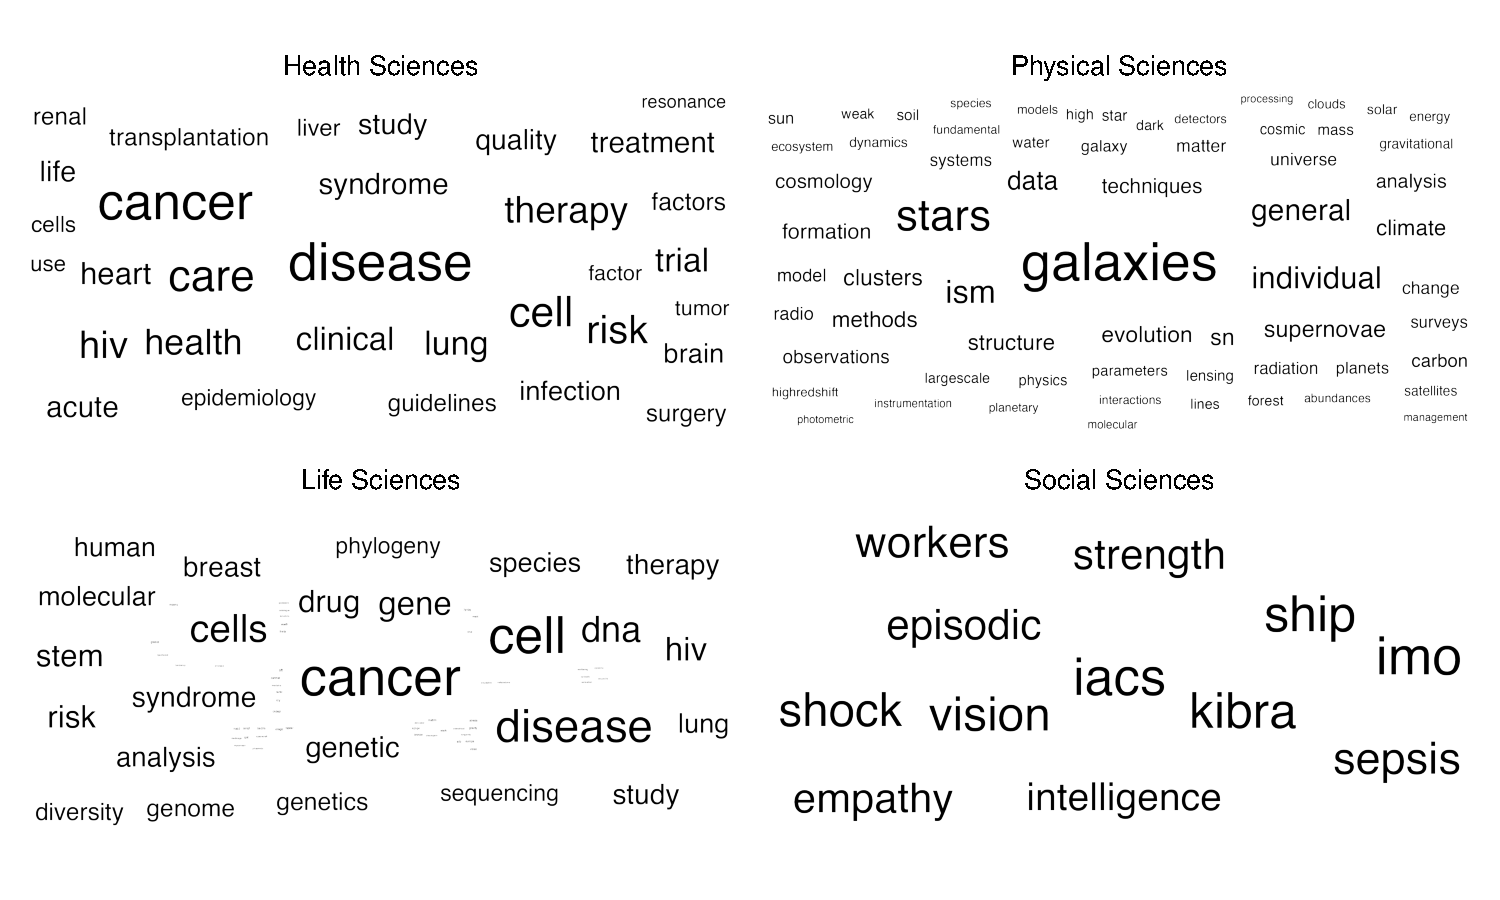
\includegraphics{manuscript_scopus_unmasked_files/figure-latex/fig-keywords-1.pdf}
\caption{\label{fig:fig-keywords}Keyword Analysis for Each of the Four Subject Areas.}
\end{figure}

\hypertarget{rq3-authors}{%
\subsection{RQ3: Authors}\label{rq3-authors}}

\hypertarget{institution}{%
\subsubsection{Institution}\label{institution}}

Institution was normalized by taking the total number of unique institutions and dividing by the total number of institution listings. The patterns are similar for each decade in that papers are often either half unique institutions or mostly unique institutions overall as shown in Figure \ref{fig:fig-inst}.

\begin{figure}
\centering
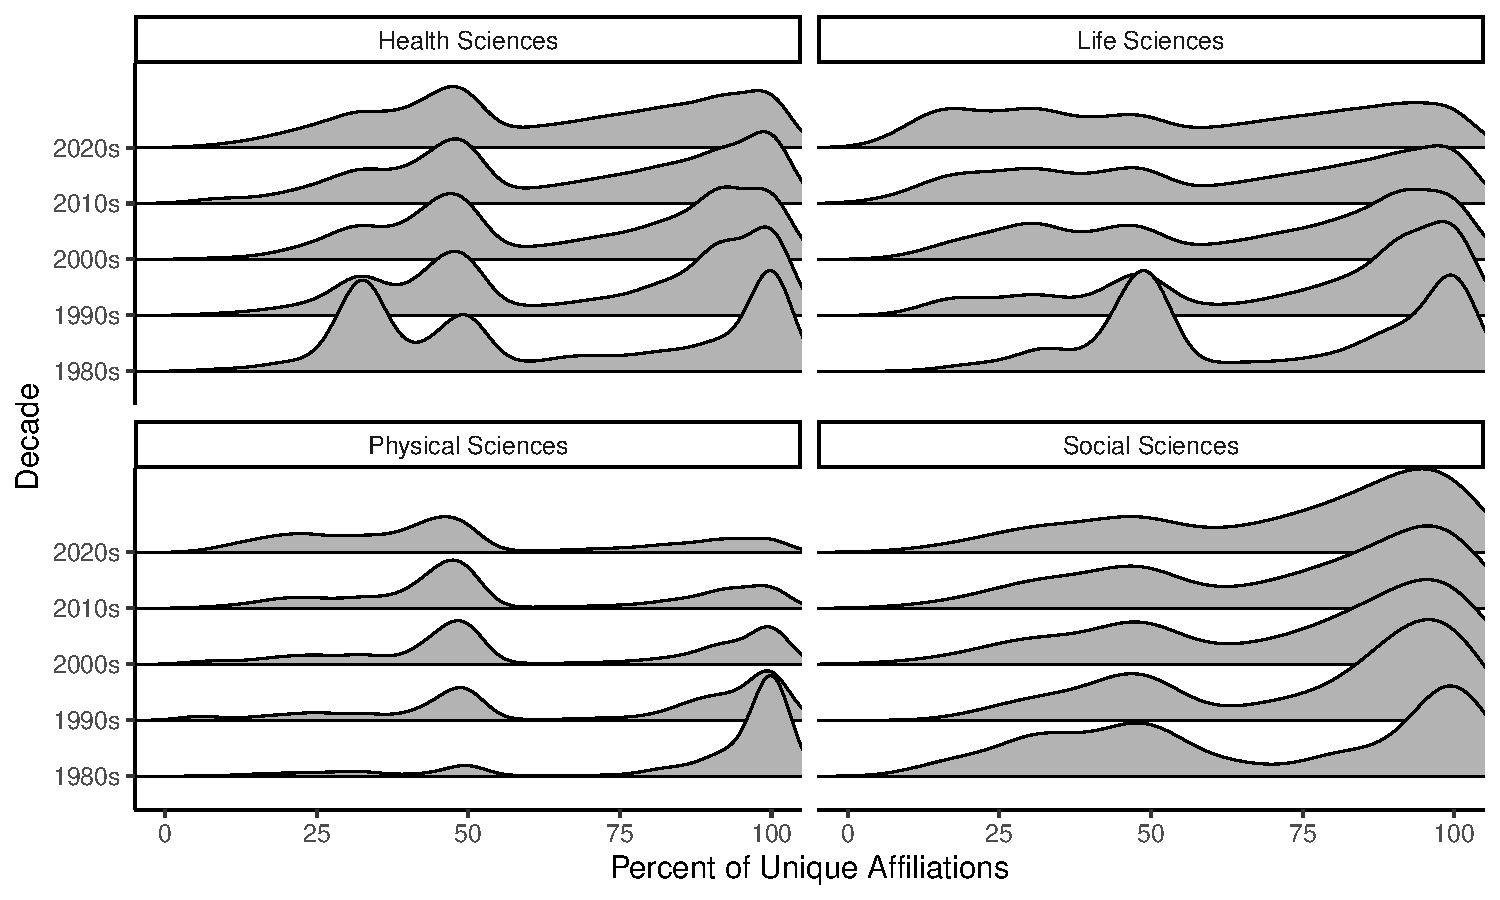
\includegraphics{manuscript_scopus_unmasked_files/figure-latex/fig-inst-1.pdf}
\caption{\label{fig:fig-inst}Number of unique institutions involved in big-team science papers across decades.}
\end{figure}

\hypertarget{education-1}{%
\subsubsection{Education}\label{education-1}}

As noted in our pre-registration, we would only present this variable if we could obtain at least 50\% information on the authors who publish in big team science papers. 95.83\% of the data was not available.

\hypertarget{types-of-publications-1}{%
\subsubsection{Types of Publications}\label{types-of-publications-1}}

Types of publications are presented in Figure \ref{fig:fig-pub-types}. The patterns of publications are roughly similar for big team science authors and all authors. It appears that proportionally, big team members are more likely to post preprints in comparison to all authors.

\begin{figure}
\centering
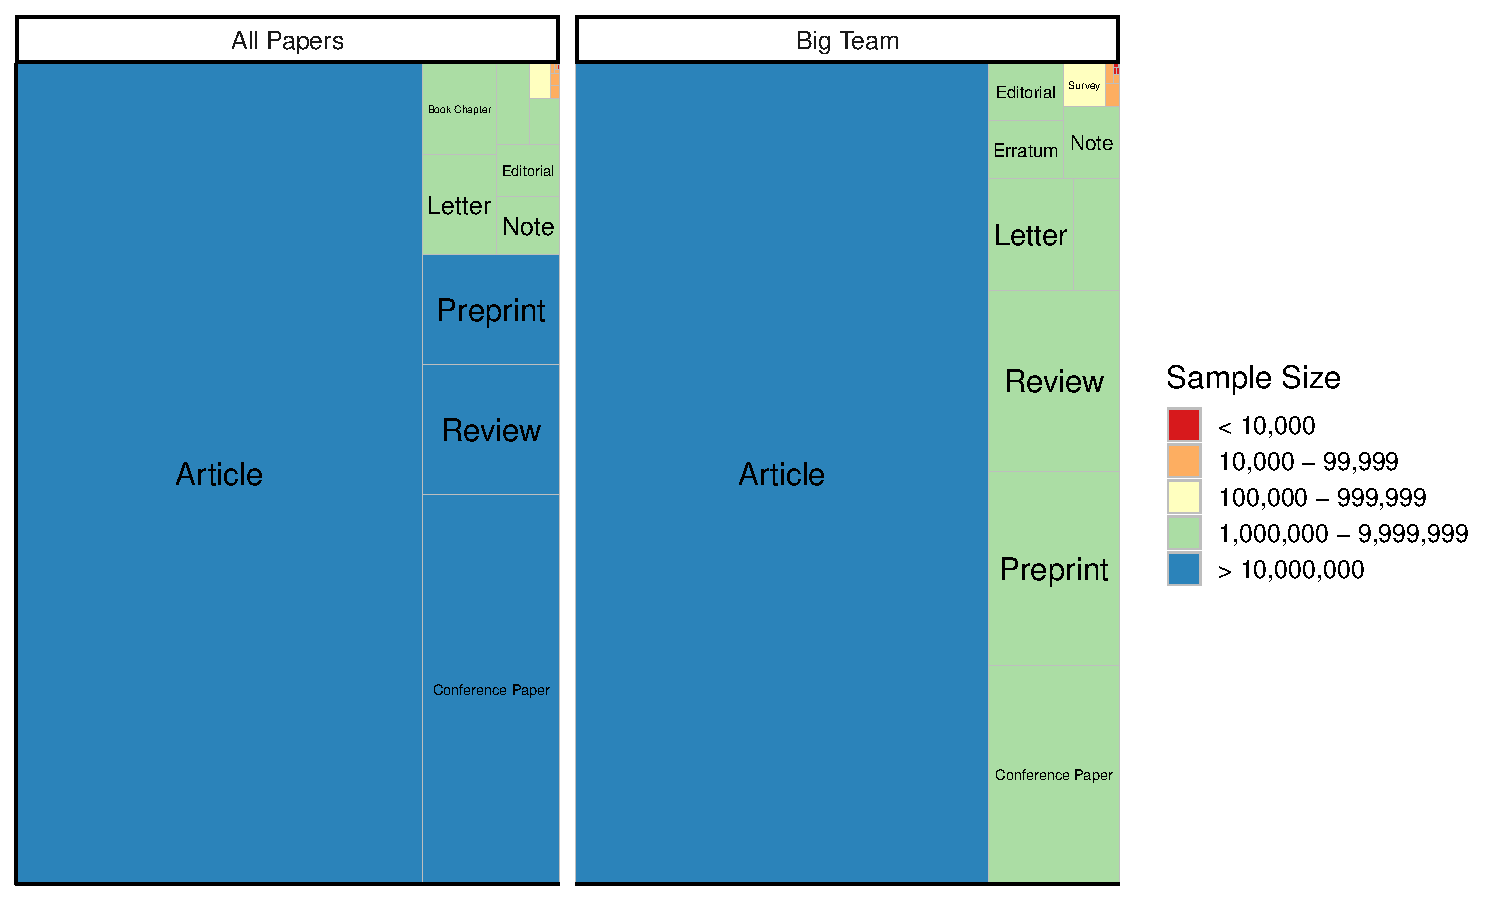
\includegraphics{manuscript_scopus_unmasked_files/figure-latex/fig-pub-types-1.pdf}
\caption{\label{fig:fig-pub-types}Types of publications for big-team science and all authors.}
\end{figure}


\end{document}
